\documentclass[1p]{elsarticle_modified}
%\bibliographystyle{elsarticle-num}

%\usepackage[colorlinks]{hyperref}
%\usepackage{abbrmath_seonhwa} %\Abb, \Ascr, \Acal ,\Abf, \Afrak
\usepackage{amsfonts}
\usepackage{amssymb}
\usepackage{amsmath}
\usepackage{amsthm}
\usepackage{scalefnt}
\usepackage{amsbsy}
\usepackage{kotex}
\usepackage{caption}
\usepackage{subfig}
\usepackage{color}
\usepackage{graphicx}
\usepackage{xcolor} %% white, black, red, green, blue, cyan, magenta, yellow
\usepackage{float}
\usepackage{setspace}
\usepackage{hyperref}

\usepackage{tikz}
\usetikzlibrary{arrows}

\usepackage{multirow}
\usepackage{array} % fixed length table
\usepackage{hhline}

%%%%%%%%%%%%%%%%%%%%%
\makeatletter
\renewcommand*\env@matrix[1][\arraystretch]{%
	\edef\arraystretch{#1}%
	\hskip -\arraycolsep
	\let\@ifnextchar\new@ifnextchar
	\array{*\c@MaxMatrixCols c}}
\makeatother %https://tex.stackexchange.com/questions/14071/how-can-i-increase-the-line-spacing-in-a-matrix
%%%%%%%%%%%%%%%

\usepackage[normalem]{ulem}

\newcommand{\msout}[1]{\ifmmode\text{\sout{\ensuremath{#1}}}\else\sout{#1}\fi}
%SOURCE: \msout is \stkout macro in https://tex.stackexchange.com/questions/20609/strikeout-in-math-mode

\newcommand{\cancel}[1]{
	\ifmmode
	{\color{red}\msout{#1}}
	\else
	{\color{red}\sout{#1}}
	\fi
}

\newcommand{\add}[1]{
	{\color{blue}\uwave{#1}}
}

\newcommand{\replace}[2]{
	\ifmmode
	{\color{red}\msout{#1}}{\color{blue}\uwave{#2}}
	\else
	{\color{red}\sout{#1}}{\color{blue}\uwave{#2}}
	\fi
}

\newcommand{\Sol}{\mathcal{S}} %segment
\newcommand{\D}{D} %diagram
\newcommand{\A}{\mathcal{A}} %arc


%%%%%%%%%%%%%%%%%%%%%%%%%%%%%5 test

\def\sl{\operatorname{\textup{SL}}(2,\Cbb)}
\def\psl{\operatorname{\textup{PSL}}(2,\Cbb)}
\def\quan{\mkern 1mu \triangleright \mkern 1mu}

\theoremstyle{definition}
\newtheorem{thm}{Theorem}[section]
\newtheorem{prop}[thm]{Proposition}
\newtheorem{lem}[thm]{Lemma}
\newtheorem{ques}[thm]{Question}
\newtheorem{cor}[thm]{Corollary}
\newtheorem{defn}[thm]{Definition}
\newtheorem{exam}[thm]{Example}
\newtheorem{rmk}[thm]{Remark}
\newtheorem{alg}[thm]{Algorithm}

\newcommand{\I}{\sqrt{-1}}
\begin{document}

%\begin{frontmatter}
%
%\title{Boundary parabolic representations of knots up to 8 crossings}
%
%%% Group authors per affiliation:
%\author{Yunhi Cho} 
%\address{Department of Mathematics, University of Seoul, Seoul, Korea}
%\ead{yhcho@uos.ac.kr}
%
%
%\author{Seonhwa Kim} %\fnref{s_kim}}
%\address{Center for Geometry and Physics, Institute for Basic Science, Pohang, 37673, Korea}
%\ead{ryeona17@ibs.re.kr}
%
%\author{Hyuk Kim}
%\address{Department of Mathematical Sciences, Seoul National University, Seoul 08826, Korea}
%\ead{hyukkim@snu.ac.kr}
%
%\author{Seokbeom Yoon}
%\address{Department of Mathematical Sciences, Seoul National University, Seoul, 08826,  Korea}
%\ead{sbyoon15@snu.ac.kr}
%
%\begin{abstract}
%We find all boundary parabolic representation of knots up to 8 crossings.
%
%\end{abstract}
%\begin{keyword}
%    \MSC[2010] 57M25 
%\end{keyword}
%
%\end{frontmatter}

%\linenumbers
%\tableofcontents
%
\newcommand\colored[1]{\textcolor{white}{\rule[-0.35ex]{0.8em}{1.4ex}}\kern-0.8em\color{red} #1}%
%\newcommand\colored[1]{\textcolor{white}{ #1}\kern-2.17ex	\textcolor{white}{ #1}\kern-1.81ex	\textcolor{white}{ #1}\kern-2.15ex\color{red}#1	}

{\Large $\underline{12a_{0309}~(K12a_{0309})}$}

\setlength{\tabcolsep}{10pt}
\renewcommand{\arraystretch}{1.6}
\vspace{1cm}\begin{tabular}{m{100pt}>{\centering\arraybackslash}m{274pt}}
\multirow{5}{120pt}{
	\centering
	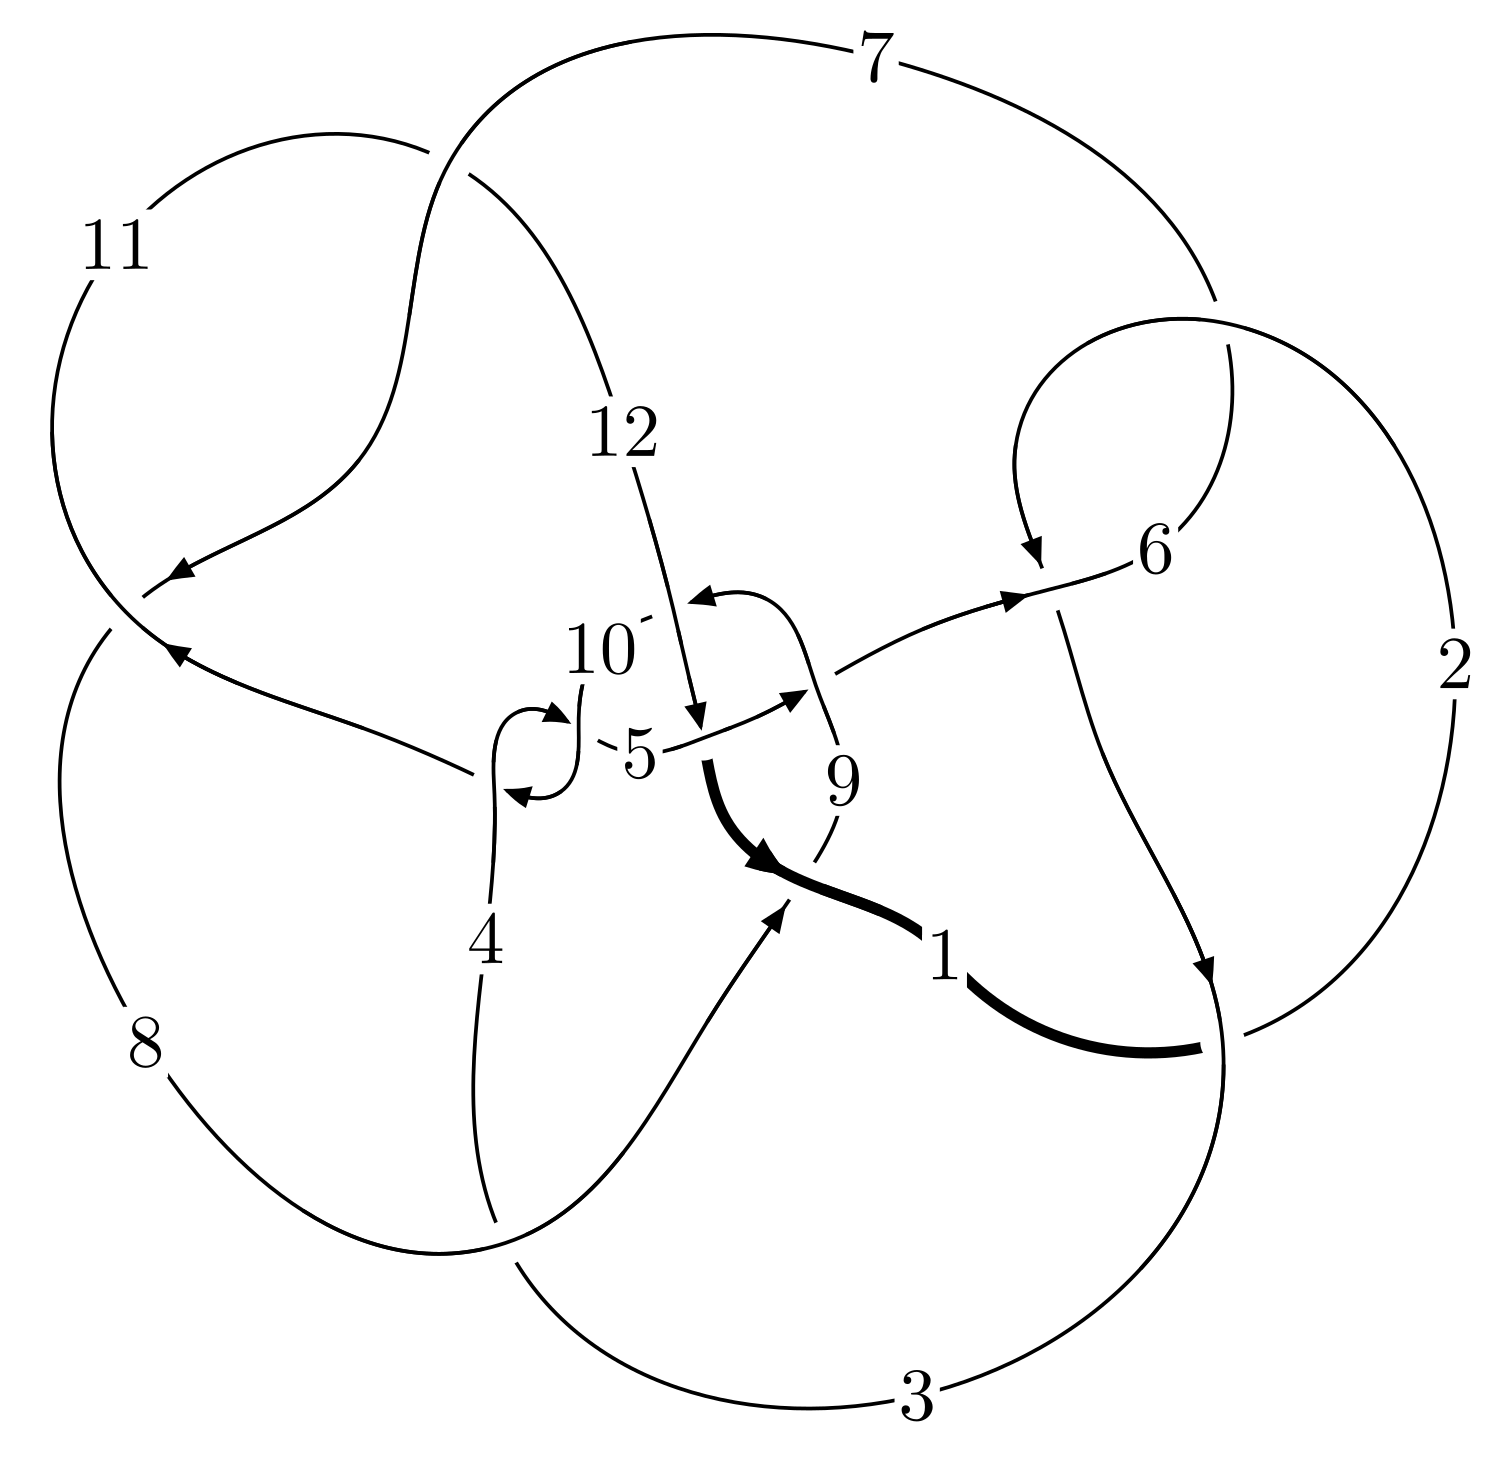
\includegraphics[width=112pt]{../../../GIT/diagram.site/Diagrams/png/1110_12a_0309.png}\\
\ \ \ A knot diagram\footnotemark}&
\allowdisplaybreaks
\textbf{Linearized knot diagam} \\
\cline{2-2}
 &
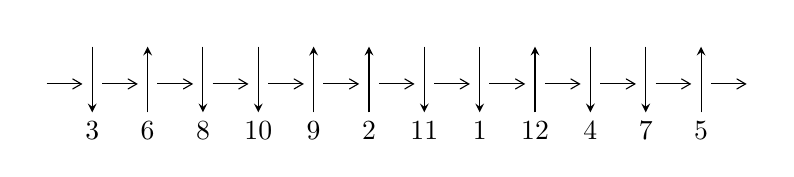
\begin{tikzpicture}[x=20pt, y=17pt]
	% nodes
	\node (C0) at (0, 0) {};
	\node (C1) at (1, 0) {};
	\node (C1U) at (1, +1) {};
	\node (C1D) at (1, -1) {3};

	\node (C2) at (2, 0) {};
	\node (C2U) at (2, +1) {};
	\node (C2D) at (2, -1) {6};

	\node (C3) at (3, 0) {};
	\node (C3U) at (3, +1) {};
	\node (C3D) at (3, -1) {8};

	\node (C4) at (4, 0) {};
	\node (C4U) at (4, +1) {};
	\node (C4D) at (4, -1) {10};

	\node (C5) at (5, 0) {};
	\node (C5U) at (5, +1) {};
	\node (C5D) at (5, -1) {9};

	\node (C6) at (6, 0) {};
	\node (C6U) at (6, +1) {};
	\node (C6D) at (6, -1) {2};

	\node (C7) at (7, 0) {};
	\node (C7U) at (7, +1) {};
	\node (C7D) at (7, -1) {11};

	\node (C8) at (8, 0) {};
	\node (C8U) at (8, +1) {};
	\node (C8D) at (8, -1) {1};

	\node (C9) at (9, 0) {};
	\node (C9U) at (9, +1) {};
	\node (C9D) at (9, -1) {12};

	\node (C10) at (10, 0) {};
	\node (C10U) at (10, +1) {};
	\node (C10D) at (10, -1) {4};

	\node (C11) at (11, 0) {};
	\node (C11U) at (11, +1) {};
	\node (C11D) at (11, -1) {7};

	\node (C12) at (12, 0) {};
	\node (C12U) at (12, +1) {};
	\node (C12D) at (12, -1) {5};
	\node (C13) at (13, 0) {};

	% arrows
	\draw[->,>={angle 60}]
	(C0) edge (C1) (C1) edge (C2) (C2) edge (C3) (C3) edge (C4) (C4) edge (C5) (C5) edge (C6) (C6) edge (C7) (C7) edge (C8) (C8) edge (C9) (C9) edge (C10) (C10) edge (C11) (C11) edge (C12) (C12) edge (C13) ;	\draw[->,>=stealth]
	(C1U) edge (C1D) (C2D) edge (C2U) (C3U) edge (C3D) (C4U) edge (C4D) (C5D) edge (C5U) (C6D) edge (C6U) (C7U) edge (C7D) (C8U) edge (C8D) (C9D) edge (C9U) (C10U) edge (C10D) (C11U) edge (C11D) (C12D) edge (C12U) ;
	\end{tikzpicture} \\
\hhline{~~} \\& 
\textbf{Solving Sequence} \\ \cline{2-2} 
 &
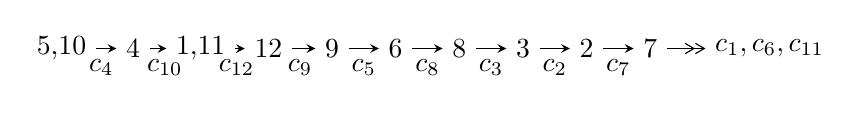
\begin{tikzpicture}[x=23pt, y=7pt]
	% node
	\node (A0) at (-1/8, 0) {5,10};
	\node (A1) at (1, 0) {4};
	\node (A2) at (33/16, 0) {1,11};
	\node (A3) at (25/8, 0) {12};
	\node (A4) at (33/8, 0) {9};
	\node (A5) at (41/8, 0) {6};
	\node (A6) at (49/8, 0) {8};
	\node (A7) at (57/8, 0) {3};
	\node (A8) at (65/8, 0) {2};
	\node (A9) at (73/8, 0) {7};
	\node (C1) at (1/2, -1) {$c_{4}$};
	\node (C2) at (3/2, -1) {$c_{10}$};
	\node (C3) at (21/8, -1) {$c_{12}$};
	\node (C4) at (29/8, -1) {$c_{9}$};
	\node (C5) at (37/8, -1) {$c_{5}$};
	\node (C6) at (45/8, -1) {$c_{8}$};
	\node (C7) at (53/8, -1) {$c_{3}$};
	\node (C8) at (61/8, -1) {$c_{2}$};
	\node (C9) at (69/8, -1) {$c_{7}$};
	\node (A10) at (11, 0) {$c_{1},c_{6},c_{11}$};

	% edge
	\draw[->,>=stealth]	
	(A0) edge (A1) (A1) edge (A2) (A2) edge (A3) (A3) edge (A4) (A4) edge (A5) (A5) edge (A6) (A6) edge (A7) (A7) edge (A8) (A8) edge (A9) ;
	\draw[->>,>={angle 60}]	
	(A9) edge (A10);
\end{tikzpicture} \\ 

\end{tabular} \\

\footnotetext{
The image of knot diagram is generated by the software ``\textbf{Draw programme}" developed by Andrew Bartholomew(\url{http://www.layer8.co.uk/maths/draw/index.htm\#Running-draw}), where we modified some parts for our purpose(\url{https://github.com/CATsTAILs/LinksPainter}).
}\phantom \\ \newline 
\centering \textbf{Ideals for irreducible components\footnotemark of $X_{\text{par}}$} 
 
\begin{align*}
I^u_{1}&=\langle 
-3.39225\times10^{858} u^{153}+1.90990\times10^{859} u^{152}+\cdots+1.42535\times10^{862} b+1.18889\times10^{864},\\
\phantom{I^u_{1}}&\phantom{= \langle  }-2.84840\times10^{864} u^{153}+5.22709\times10^{864} u^{152}+\cdots+1.60581\times10^{867} a+7.40412\times10^{868},\\
\phantom{I^u_{1}}&\phantom{= \langle  }u^{154}- u^{153}+\cdots-1143847 u+112661\rangle \\
I^u_{2}&=\langle 
-4.22889\times10^{38} u^{45}-7.22511\times10^{39} u^{44}+\cdots+4.86508\times10^{38} b-1.65490\times10^{40},\\
\phantom{I^u_{2}}&\phantom{= \langle  }-2.30560\times10^{40} u^{45}-1.40190\times10^{40} u^{44}+\cdots+1.45952\times10^{39} a-3.45185\times10^{40},\\
\phantom{I^u_{2}}&\phantom{= \langle  }u^{46}+21 u^{44}+\cdots+3 u+1\rangle \\
I^u_{3}&=\langle 
b- u,\;a,\;u^{14}+2 u^{12}+u^{10}+2 u^8+u^7+2 u^6+u^5+u^2+u+1\rangle \\
\\
\end{align*}
\raggedright * 3 irreducible components of $\dim_{\mathbb{C}}=0$, with total 214 representations.\\
\footnotetext{All coefficients of polynomials are rational numbers. But the coefficients are sometimes approximated in decimal forms when there is not enough margin.}
\newpage
\renewcommand{\arraystretch}{1}
\centering \section*{I. $I^u_{1}= \langle -3.39\times10^{858} u^{153}+1.91\times10^{859} u^{152}+\cdots+1.43\times10^{862} b+1.19\times10^{864},\;-2.85\times10^{864} u^{153}+5.23\times10^{864} u^{152}+\cdots+1.61\times10^{867} a+7.40\times10^{868},\;u^{154}- u^{153}+\cdots-1143847 u+112661 \rangle$}
\flushleft \textbf{(i) Arc colorings}\\
\begin{tabular}{m{7pt} m{180pt} m{7pt} m{180pt} }
\flushright $a_{5}=$&$\begin{pmatrix}1\\0\end{pmatrix}$ \\
\flushright $a_{10}=$&$\begin{pmatrix}0\\u\end{pmatrix}$ \\
\flushright $a_{4}=$&$\begin{pmatrix}1\\- u^2\end{pmatrix}$ \\
\flushright $a_{1}=$&$\begin{pmatrix}0.00177381 u^{153}-0.00325511 u^{152}+\cdots+671.644 u-46.1082\\0.000237994 u^{153}-0.00133995 u^{152}+\cdots+878.554 u-83.4103\end{pmatrix}$ \\
\flushright $a_{11}=$&$\begin{pmatrix}- u\\u^3+u\end{pmatrix}$ \\
\flushright $a_{12}=$&$\begin{pmatrix}0.00153581 u^{153}-0.00191516 u^{152}+\cdots-206.910 u+37.3021\\0.000237994 u^{153}-0.00133995 u^{152}+\cdots+878.554 u-83.4103\end{pmatrix}$ \\
\flushright $a_{9}=$&$\begin{pmatrix}0.000939431 u^{153}-0.00110689 u^{152}+\cdots+184.723 u-17.1986\\-0.000532150 u^{153}+0.000211654 u^{152}+\cdots+335.198 u-37.4226\end{pmatrix}$ \\
\flushright $a_{6}=$&$\begin{pmatrix}-0.000256300 u^{153}-0.00305237 u^{152}+\cdots+2848.54 u-284.248\\-0.00120465 u^{153}+0.000746461 u^{152}+\cdots+591.126 u-66.7312\end{pmatrix}$ \\
\flushright $a_{8}=$&$\begin{pmatrix}-0.000589338 u^{153}+0.0000342459 u^{152}+\cdots+517.802 u-53.6851\\-0.00118166 u^{153}+0.00183121 u^{152}+\cdots-408.716 u+32.7101\end{pmatrix}$ \\
\flushright $a_{3}=$&$\begin{pmatrix}-0.000292379 u^{153}+0.00194373 u^{152}+\cdots-1479.75 u+144.955\\0.000567327 u^{153}-0.00126130 u^{152}+\cdots+462.941 u-40.9968\end{pmatrix}$ \\
\flushright $a_{2}=$&$\begin{pmatrix}0.00333143 u^{153}-0.00305964 u^{152}+\cdots-907.570 u+112.824\\0.00109675 u^{153}-0.00365980 u^{152}+\cdots+1903.93 u-177.939\end{pmatrix}$ \\
\flushright $a_{7}=$&$\begin{pmatrix}0.000231030 u^{153}-0.00199593 u^{152}+\cdots+1354.30 u-128.116\\-0.00114791 u^{153}+0.00101689 u^{152}+\cdots+231.045 u-29.1577\end{pmatrix}$\\&\end{tabular}
\flushleft \textbf{(ii) Obstruction class $= -1$}\\~\\
\flushleft \textbf{(iii) Cusp Shapes $= -0.00225151 u^{153}+0.00479437 u^{152}+\cdots-2232.62 u+208.796$}\\~\\
\newpage\renewcommand{\arraystretch}{1}
\flushleft \textbf{(iv) u-Polynomials at the component}\newline \\
\begin{tabular}{m{50pt}|m{274pt}}
Crossings & \hspace{64pt}u-Polynomials at each crossing \\
\hline $$\begin{aligned}c_{1}\end{aligned}$$&$\begin{aligned}
&u^{154}+70 u^{153}+\cdots+2351600 u+40000
\end{aligned}$\\
\hline $$\begin{aligned}c_{2},c_{6}\end{aligned}$$&$\begin{aligned}
&u^{154}+4 u^{153}+\cdots+2700 u+200
\end{aligned}$\\
\hline $$\begin{aligned}c_{3}\end{aligned}$$&$\begin{aligned}
&u^{154}- u^{153}+\cdots+2016184651 u+1384157231
\end{aligned}$\\
\hline $$\begin{aligned}c_{4},c_{10}\end{aligned}$$&$\begin{aligned}
&u^{154}- u^{153}+\cdots-1143847 u+112661
\end{aligned}$\\
\hline $$\begin{aligned}c_{5}\end{aligned}$$&$\begin{aligned}
&u^{154}-4 u^{153}+\cdots+55 u+1
\end{aligned}$\\
\hline $$\begin{aligned}c_{7},c_{11}\end{aligned}$$&$\begin{aligned}
&u^{154}+2 u^{153}+\cdots-249479005 u+13493731
\end{aligned}$\\
\hline $$\begin{aligned}c_{8}\end{aligned}$$&$\begin{aligned}
&u^{154}+9 u^{153}+\cdots-649198290 u+29322847
\end{aligned}$\\
\hline $$\begin{aligned}c_{9}\end{aligned}$$&$\begin{aligned}
&u^{154}+18 u^{153}+\cdots+290880 u+11897
\end{aligned}$\\
\hline $$\begin{aligned}c_{12}\end{aligned}$$&$\begin{aligned}
&u^{154}-20 u^{152}+\cdots-232062 u+57347
\end{aligned}$\\
\hline
\end{tabular}\\~\\
\newpage\renewcommand{\arraystretch}{1}
\flushleft \textbf{(v) Riley Polynomials at the component}\newline \\
\begin{tabular}{m{50pt}|m{274pt}}
Crossings & \hspace{64pt}Riley Polynomials at each crossing \\
\hline $$\begin{aligned}c_{1}\end{aligned}$$&$\begin{aligned}
&y^{154}+46 y^{153}+\cdots+924906720000 y+1600000000
\end{aligned}$\\
\hline $$\begin{aligned}c_{2},c_{6}\end{aligned}$$&$\begin{aligned}
&y^{154}+70 y^{153}+\cdots+2351600 y+40000
\end{aligned}$\\
\hline $$\begin{aligned}c_{3}\end{aligned}$$&$\begin{aligned}
&y^{154}+63 y^{153}+\cdots-3.46\times10^{19} y+1.92\times10^{18}
\end{aligned}$\\
\hline $$\begin{aligned}c_{4},c_{10}\end{aligned}$$&$\begin{aligned}
&y^{154}+139 y^{153}+\cdots-104773968485 y+12692500921
\end{aligned}$\\
\hline $$\begin{aligned}c_{5}\end{aligned}$$&$\begin{aligned}
&y^{154}+6 y^{153}+\cdots-143 y+1
\end{aligned}$\\
\hline $$\begin{aligned}c_{7},c_{11}\end{aligned}$$&$\begin{aligned}
&y^{154}+114 y^{153}+\cdots+2908457925570425 y+182080776300361
\end{aligned}$\\
\hline $$\begin{aligned}c_{8}\end{aligned}$$&$\begin{aligned}
&y^{154}+37 y^{153}+\cdots+16647274284827280 y+859829356185409
\end{aligned}$\\
\hline $$\begin{aligned}c_{9}\end{aligned}$$&$\begin{aligned}
&y^{154}-34 y^{153}+\cdots-6991839034 y+141538609
\end{aligned}$\\
\hline $$\begin{aligned}c_{12}\end{aligned}$$&$\begin{aligned}
&y^{154}-40 y^{153}+\cdots-208157950460 y+3288678409
\end{aligned}$\\
\hline
\end{tabular}\\~\\
\newpage\flushleft \textbf{(vi) Complex Volumes and Cusp Shapes}
$$\begin{array}{c|c|c}  
\text{Solutions to }I^u_{1}& \I (\text{vol} + \sqrt{-1}CS) & \text{Cusp shape}\\
 \hline 
\begin{aligned}
u &= \phantom{-}0.680276 + 0.738161 I \\
a &= -1.357200 - 0.079694 I \\
b &= -1.019250 + 0.939094 I\end{aligned}
 & -3.82081 - 4.81342 I & \phantom{-0.000000 } 0 \\ \hline\begin{aligned}
u &= \phantom{-}0.680276 - 0.738161 I \\
a &= -1.357200 + 0.079694 I \\
b &= -1.019250 - 0.939094 I\end{aligned}
 & -3.82081 + 4.81342 I & \phantom{-0.000000 } 0 \\ \hline\begin{aligned}
u &= \phantom{-}0.504148 + 0.841661 I \\
a &= -1.55694 - 1.18967 I \\
b &= -0.961833 + 0.610685 I\end{aligned}
 & \phantom{-}0.64778 - 3.05199 I & \phantom{-0.000000 } 0 \\ \hline\begin{aligned}
u &= \phantom{-}0.504148 - 0.841661 I \\
a &= -1.55694 + 1.18967 I \\
b &= -0.961833 - 0.610685 I\end{aligned}
 & \phantom{-}0.64778 + 3.05199 I & \phantom{-0.000000 } 0 \\ \hline\begin{aligned}
u &= -0.285517 + 0.927898 I \\
a &= \phantom{-}2.35344 - 0.97712 I \\
b &= \phantom{-}1.080010 + 0.419366 I\end{aligned}
 & \phantom{-}0.18002 + 6.26907 I & \phantom{-0.000000 } 0 \\ \hline\begin{aligned}
u &= -0.285517 - 0.927898 I \\
a &= \phantom{-}2.35344 + 0.97712 I \\
b &= \phantom{-}1.080010 - 0.419366 I\end{aligned}
 & \phantom{-}0.18002 - 6.26907 I & \phantom{-0.000000 } 0 \\ \hline\begin{aligned}
u &= -0.610780 + 0.742892 I \\
a &= -2.09941 - 0.95812 I \\
b &= -1.75886 - 1.25119 I\end{aligned}
 & -1.34690 + 2.43834 I & \phantom{-0.000000 } 0 \\ \hline\begin{aligned}
u &= -0.610780 - 0.742892 I \\
a &= -2.09941 + 0.95812 I \\
b &= -1.75886 + 1.25119 I\end{aligned}
 & -1.34690 - 2.43834 I & \phantom{-0.000000 } 0 \\ \hline\begin{aligned}
u &= -0.300717 + 0.908720 I \\
a &= \phantom{-}1.062630 - 0.089277 I \\
b &= \phantom{-}0.744562 + 0.867791 I\end{aligned}
 & \phantom{-}0.68630 + 2.30026 I & \phantom{-0.000000 } 0 \\ \hline\begin{aligned}
u &= -0.300717 - 0.908720 I \\
a &= \phantom{-}1.062630 + 0.089277 I \\
b &= \phantom{-}0.744562 - 0.867791 I\end{aligned}
 & \phantom{-}0.68630 - 2.30026 I & \phantom{-0.000000 } 0\\
 \hline 
 \end{array}$$\newpage$$\begin{array}{c|c|c}  
\text{Solutions to }I^u_{1}& \I (\text{vol} + \sqrt{-1}CS) & \text{Cusp shape}\\
 \hline 
\begin{aligned}
u &= \phantom{-}0.385458 + 0.850098 I \\
a &= \phantom{-}0.097392 + 1.025470 I \\
b &= \phantom{-}0.448483 + 1.102820 I\end{aligned}
 & -3.41216 + 0.66021 I & \phantom{-0.000000 } 0 \\ \hline\begin{aligned}
u &= \phantom{-}0.385458 - 0.850098 I \\
a &= \phantom{-}0.097392 - 1.025470 I \\
b &= \phantom{-}0.448483 - 1.102820 I\end{aligned}
 & -3.41216 - 0.66021 I & \phantom{-0.000000 } 0 \\ \hline\begin{aligned}
u &= -0.110996 + 1.083840 I \\
a &= -0.138900 + 0.057689 I \\
b &= -0.629890 - 0.584548 I\end{aligned}
 & \phantom{-}1.32837 - 5.00544 I & \phantom{-0.000000 } 0 \\ \hline\begin{aligned}
u &= -0.110996 - 1.083840 I \\
a &= -0.138900 - 0.057689 I \\
b &= -0.629890 + 0.584548 I\end{aligned}
 & \phantom{-}1.32837 + 5.00544 I & \phantom{-0.000000 } 0 \\ \hline\begin{aligned}
u &= -0.096899 + 1.146000 I \\
a &= \phantom{-}2.75265 - 0.12374 I \\
b &= \phantom{-}1.74385 - 0.15037 I\end{aligned}
 & \phantom{-}1.26900 - 1.14595 I & \phantom{-0.000000 } 0 \\ \hline\begin{aligned}
u &= -0.096899 - 1.146000 I \\
a &= \phantom{-}2.75265 + 0.12374 I \\
b &= \phantom{-}1.74385 + 0.15037 I\end{aligned}
 & \phantom{-}1.26900 + 1.14595 I & \phantom{-0.000000 } 0 \\ \hline\begin{aligned}
u &= -0.844043 + 0.048061 I \\
a &= -0.217403 + 0.102016 I \\
b &= -0.811064 + 0.891451 I\end{aligned}
 & -4.46898 - 1.86070 I & \phantom{-0.000000 } 0 \\ \hline\begin{aligned}
u &= -0.844043 - 0.048061 I \\
a &= -0.217403 - 0.102016 I \\
b &= -0.811064 - 0.891451 I\end{aligned}
 & -4.46898 + 1.86070 I & \phantom{-0.000000 } 0 \\ \hline\begin{aligned}
u &= -0.825409 + 0.082473 I \\
a &= -1.49726 + 0.21682 I \\
b &= -0.943008 - 0.954276 I\end{aligned}
 & \phantom{-}1.87730 - 7.43583 I & \phantom{-0.000000 } 0 \\ \hline\begin{aligned}
u &= -0.825409 - 0.082473 I \\
a &= -1.49726 - 0.21682 I \\
b &= -0.943008 + 0.954276 I\end{aligned}
 & \phantom{-}1.87730 + 7.43583 I & \phantom{-0.000000 } 0\\
 \hline 
 \end{array}$$\newpage$$\begin{array}{c|c|c}  
\text{Solutions to }I^u_{1}& \I (\text{vol} + \sqrt{-1}CS) & \text{Cusp shape}\\
 \hline 
\begin{aligned}
u &= \phantom{-}0.028330 + 1.171140 I \\
a &= \phantom{-}0.82002 + 2.31604 I \\
b &= \phantom{-}0.82307 + 2.55897 I\end{aligned}
 & \phantom{-}1.26673 - 3.35634 I & \phantom{-0.000000 } 0 \\ \hline\begin{aligned}
u &= \phantom{-}0.028330 - 1.171140 I \\
a &= \phantom{-}0.82002 - 2.31604 I \\
b &= \phantom{-}0.82307 - 2.55897 I\end{aligned}
 & \phantom{-}1.26673 + 3.35634 I & \phantom{-0.000000 } 0 \\ \hline\begin{aligned}
u &= -0.648227 + 0.510501 I \\
a &= -0.706411 - 0.373495 I \\
b &= \phantom{-}0.839916 - 0.303316 I\end{aligned}
 & \phantom{-}0.10185 - 6.51912 I & \phantom{-0.000000 } 0 \\ \hline\begin{aligned}
u &= -0.648227 - 0.510501 I \\
a &= -0.706411 + 0.373495 I \\
b &= \phantom{-}0.839916 + 0.303316 I\end{aligned}
 & \phantom{-}0.10185 + 6.51912 I & \phantom{-0.000000 } 0 \\ \hline\begin{aligned}
u &= \phantom{-}0.739790 + 0.347254 I \\
a &= \phantom{-}0.669955 - 0.037100 I \\
b &= -0.793443 - 0.224422 I\end{aligned}
 & \phantom{-}1.28293 + 2.27410 I & \phantom{-0.000000 } 0 \\ \hline\begin{aligned}
u &= \phantom{-}0.739790 - 0.347254 I \\
a &= \phantom{-}0.669955 + 0.037100 I \\
b &= -0.793443 + 0.224422 I\end{aligned}
 & \phantom{-}1.28293 - 2.27410 I & \phantom{-0.000000 } 0 \\ \hline\begin{aligned}
u &= \phantom{-}0.598042 + 1.021020 I \\
a &= -1.27886 - 0.78167 I \\
b &= -1.049090 + 0.667325 I\end{aligned}
 & \phantom{-}1.77046 - 7.34207 I & \phantom{-0.000000 } 0 \\ \hline\begin{aligned}
u &= \phantom{-}0.598042 - 1.021020 I \\
a &= -1.27886 + 0.78167 I \\
b &= -1.049090 - 0.667325 I\end{aligned}
 & \phantom{-}1.77046 + 7.34207 I & \phantom{-0.000000 } 0 \\ \hline\begin{aligned}
u &= -0.538039 + 1.073050 I \\
a &= \phantom{-}1.27668 - 0.62270 I \\
b &= \phantom{-}1.037410 + 0.638222 I\end{aligned}
 & \phantom{-}2.32181 + 2.85382 I & \phantom{-0.000000 } 0 \\ \hline\begin{aligned}
u &= -0.538039 - 1.073050 I \\
a &= \phantom{-}1.27668 + 0.62270 I \\
b &= \phantom{-}1.037410 - 0.638222 I\end{aligned}
 & \phantom{-}2.32181 - 2.85382 I & \phantom{-0.000000 } 0\\
 \hline 
 \end{array}$$\newpage$$\begin{array}{c|c|c}  
\text{Solutions to }I^u_{1}& \I (\text{vol} + \sqrt{-1}CS) & \text{Cusp shape}\\
 \hline 
\begin{aligned}
u &= -0.250880 + 1.176150 I \\
a &= -1.47255 + 1.02922 I \\
b &= -0.960814 - 0.615935 I\end{aligned}
 & \phantom{-}2.22996 + 9.76512 I & \phantom{-0.000000 } 0 \\ \hline\begin{aligned}
u &= -0.250880 - 1.176150 I \\
a &= -1.47255 - 1.02922 I \\
b &= -0.960814 + 0.615935 I\end{aligned}
 & \phantom{-}2.22996 - 9.76512 I & \phantom{-0.000000 } 0 \\ \hline\begin{aligned}
u &= -0.150902 + 1.197400 I \\
a &= -1.87161 + 0.75958 I \\
b &= -1.041870 - 0.664675 I\end{aligned}
 & \phantom{-}1.33987 + 2.44790 I & \phantom{-0.000000 } 0 \\ \hline\begin{aligned}
u &= -0.150902 - 1.197400 I \\
a &= -1.87161 - 0.75958 I \\
b &= -1.041870 + 0.664675 I\end{aligned}
 & \phantom{-}1.33987 - 2.44790 I & \phantom{-0.000000 } 0 \\ \hline\begin{aligned}
u &= \phantom{-}0.213634 + 1.193460 I \\
a &= \phantom{-}0.494881 - 0.200383 I \\
b &= \phantom{-}0.701619 - 0.724730 I\end{aligned}
 & \phantom{-}4.05101 + 0.41529 I & \phantom{-0.000000 } 0 \\ \hline\begin{aligned}
u &= \phantom{-}0.213634 - 1.193460 I \\
a &= \phantom{-}0.494881 + 0.200383 I \\
b &= \phantom{-}0.701619 + 0.724730 I\end{aligned}
 & \phantom{-}4.05101 - 0.41529 I & \phantom{-0.000000 } 0 \\ \hline\begin{aligned}
u &= \phantom{-}0.176146 + 1.208500 I \\
a &= -2.46754 + 0.14885 I \\
b &= -1.82483 + 0.65605 I\end{aligned}
 & \phantom{-}4.34975 - 3.97955 I & \phantom{-0.000000 } 0 \\ \hline\begin{aligned}
u &= \phantom{-}0.176146 - 1.208500 I \\
a &= -2.46754 - 0.14885 I \\
b &= -1.82483 - 0.65605 I\end{aligned}
 & \phantom{-}4.34975 + 3.97955 I & \phantom{-0.000000 } 0 \\ \hline\begin{aligned}
u &= -0.409723 + 1.154180 I \\
a &= -0.234750 - 0.814571 I \\
b &= -0.264992 - 1.053720 I\end{aligned}
 & -0.58320 + 3.01376 I & \phantom{-0.000000 } 0 \\ \hline\begin{aligned}
u &= -0.409723 - 1.154180 I \\
a &= -0.234750 + 0.814571 I \\
b &= -0.264992 + 1.053720 I\end{aligned}
 & -0.58320 - 3.01376 I & \phantom{-0.000000 } 0\\
 \hline 
 \end{array}$$\newpage$$\begin{array}{c|c|c}  
\text{Solutions to }I^u_{1}& \I (\text{vol} + \sqrt{-1}CS) & \text{Cusp shape}\\
 \hline 
\begin{aligned}
u &= -0.155735 + 1.218650 I \\
a &= \phantom{-}0.969284 - 0.800962 I \\
b &= \phantom{-}0.484991 + 0.217555 I\end{aligned}
 & \phantom{-}0.70263 + 1.39575 I & \phantom{-0.000000 } 0 \\ \hline\begin{aligned}
u &= -0.155735 - 1.218650 I \\
a &= \phantom{-}0.969284 + 0.800962 I \\
b &= \phantom{-}0.484991 - 0.217555 I\end{aligned}
 & \phantom{-}0.70263 - 1.39575 I & \phantom{-0.000000 } 0 \\ \hline\begin{aligned}
u &= -0.751725 + 0.135973 I \\
a &= -0.002277 + 0.176126 I \\
b &= -0.922149 - 0.840079 I\end{aligned}
 & -1.18918 + 9.46525 I & \phantom{-0.000000 } 0 \\ \hline\begin{aligned}
u &= -0.751725 - 0.135973 I \\
a &= -0.002277 - 0.176126 I \\
b &= -0.922149 + 0.840079 I\end{aligned}
 & -1.18918 - 9.46525 I & \phantom{-0.000000 } 0 \\ \hline\begin{aligned}
u &= -0.186399 + 1.248160 I \\
a &= \phantom{-}1.96091 + 1.45626 I \\
b &= \phantom{-}0.609034 - 0.093752 I\end{aligned}
 & \phantom{-}7.81077 + 9.34359 I & \phantom{-0.000000 } 0 \\ \hline\begin{aligned}
u &= -0.186399 - 1.248160 I \\
a &= \phantom{-}1.96091 - 1.45626 I \\
b &= \phantom{-}0.609034 + 0.093752 I\end{aligned}
 & \phantom{-}7.81077 - 9.34359 I & \phantom{-0.000000 } 0 \\ \hline\begin{aligned}
u &= -0.109360 + 1.274490 I \\
a &= \phantom{-}1.26238 + 0.85032 I \\
b &= \phantom{-}0.731284 - 0.262524 I\end{aligned}
 & \phantom{-}4.64815 + 2.86380 I & \phantom{-0.000000 } 0 \\ \hline\begin{aligned}
u &= -0.109360 - 1.274490 I \\
a &= \phantom{-}1.26238 - 0.85032 I \\
b &= \phantom{-}0.731284 + 0.262524 I\end{aligned}
 & \phantom{-}4.64815 - 2.86380 I & \phantom{-0.000000 } 0 \\ \hline\begin{aligned}
u &= \phantom{-}0.222707 + 1.261150 I \\
a &= \phantom{-}1.47489 + 0.69500 I \\
b &= \phantom{-}0.924337 - 0.691392 I\end{aligned}
 & \phantom{-}4.63470 - 5.73526 I & \phantom{-0.000000 } 0 \\ \hline\begin{aligned}
u &= \phantom{-}0.222707 - 1.261150 I \\
a &= \phantom{-}1.47489 - 0.69500 I \\
b &= \phantom{-}0.924337 + 0.691392 I\end{aligned}
 & \phantom{-}4.63470 + 5.73526 I & \phantom{-0.000000 } 0\\
 \hline 
 \end{array}$$\newpage$$\begin{array}{c|c|c}  
\text{Solutions to }I^u_{1}& \I (\text{vol} + \sqrt{-1}CS) & \text{Cusp shape}\\
 \hline 
\begin{aligned}
u &= \phantom{-}0.704061 + 0.123618 I \\
a &= \phantom{-}1.88251 + 0.13761 I \\
b &= \phantom{-}0.990278 - 0.857898 I\end{aligned}
 & \phantom{-}4.23750 + 1.62869 I & \phantom{-0.000000 } 0 \\ \hline\begin{aligned}
u &= \phantom{-}0.704061 - 0.123618 I \\
a &= \phantom{-}1.88251 - 0.13761 I \\
b &= \phantom{-}0.990278 + 0.857898 I\end{aligned}
 & \phantom{-}4.23750 - 1.62869 I & \phantom{-0.000000 } 0 \\ \hline\begin{aligned}
u &= \phantom{-}0.193314 + 1.271610 I \\
a &= -2.05285 + 1.13190 I \\
b &= -0.670798 - 0.064763 I\end{aligned}
 & \phantom{-}9.49465 - 4.18882 I & \phantom{-0.000000 } 0 \\ \hline\begin{aligned}
u &= \phantom{-}0.193314 - 1.271610 I \\
a &= -2.05285 - 1.13190 I \\
b &= -0.670798 + 0.064763 I\end{aligned}
 & \phantom{-}9.49465 + 4.18882 I & \phantom{-0.000000 } 0 \\ \hline\begin{aligned}
u &= \phantom{-}0.323783 + 1.250010 I \\
a &= -0.65894 - 1.57180 I \\
b &= -0.72310 - 1.97844 I\end{aligned}
 & \phantom{-}7.73141 - 5.42666 I & \phantom{-0.000000 } 0 \\ \hline\begin{aligned}
u &= \phantom{-}0.323783 - 1.250010 I \\
a &= -0.65894 + 1.57180 I \\
b &= -0.72310 + 1.97844 I\end{aligned}
 & \phantom{-}7.73141 + 5.42666 I & \phantom{-0.000000 } 0 \\ \hline\begin{aligned}
u &= -0.378323 + 1.241380 I \\
a &= \phantom{-}1.97051 - 0.14474 I \\
b &= \phantom{-}1.30514 + 0.80182 I\end{aligned}
 & -0.74937 + 6.21479 I & \phantom{-0.000000 } 0 \\ \hline\begin{aligned}
u &= -0.378323 - 1.241380 I \\
a &= \phantom{-}1.97051 + 0.14474 I \\
b &= \phantom{-}1.30514 - 0.80182 I\end{aligned}
 & -0.74937 - 6.21479 I & \phantom{-0.000000 } 0 \\ \hline\begin{aligned}
u &= -0.597108 + 0.363941 I \\
a &= \phantom{-}0.52684 - 1.70497 I \\
b &= \phantom{-}0.586518 + 0.608844 I\end{aligned}
 & -0.30752 + 6.59655 I & \phantom{-0.000000 } 0. - 11.22925 I \\ \hline\begin{aligned}
u &= -0.597108 - 0.363941 I \\
a &= \phantom{-}0.52684 + 1.70497 I \\
b &= \phantom{-}0.586518 - 0.608844 I\end{aligned}
 & -0.30752 - 6.59655 I & \phantom{-0.000000 -}0. + 11.22925 I\\
 \hline 
 \end{array}$$\newpage$$\begin{array}{c|c|c}  
\text{Solutions to }I^u_{1}& \I (\text{vol} + \sqrt{-1}CS) & \text{Cusp shape}\\
 \hline 
\begin{aligned}
u &= \phantom{-}0.688105 + 0.075351 I \\
a &= -0.0773368 + 0.0429747 I \\
b &= \phantom{-}0.893669 - 0.808821 I\end{aligned}
 & \phantom{-}0.76910 - 4.17192 I & \phantom{-0.000000 -}0. + 2.96945 I \\ \hline\begin{aligned}
u &= \phantom{-}0.688105 - 0.075351 I \\
a &= -0.0773368 - 0.0429747 I \\
b &= \phantom{-}0.893669 + 0.808821 I\end{aligned}
 & \phantom{-}0.76910 + 4.17192 I & \phantom{-0.000000 } 0. - 2.96945 I \\ \hline\begin{aligned}
u &= \phantom{-}1.268200 + 0.323241 I \\
a &= -0.563489 - 0.040982 I \\
b &= -0.965910 + 0.857200 I\end{aligned}
 & \phantom{-}2.0993 - 14.0844 I & \phantom{-0.000000 } 0 \\ \hline\begin{aligned}
u &= \phantom{-}1.268200 - 0.323241 I \\
a &= -0.563489 + 0.040982 I \\
b &= -0.965910 - 0.857200 I\end{aligned}
 & \phantom{-}2.0993 + 14.0844 I & \phantom{-0.000000 } 0 \\ \hline\begin{aligned}
u &= -0.644823 + 0.248468 I \\
a &= \phantom{-}0.519385 - 1.059250 I \\
b &= \phantom{-}0.249825 + 0.560299 I\end{aligned}
 & -1.62100 + 1.20613 I & -7.60402 - 3.45153 I \\ \hline\begin{aligned}
u &= -0.644823 - 0.248468 I \\
a &= \phantom{-}0.519385 + 1.059250 I \\
b &= \phantom{-}0.249825 - 0.560299 I\end{aligned}
 & -1.62100 - 1.20613 I & -7.60402 + 3.45153 I \\ \hline\begin{aligned}
u &= \phantom{-}0.197940 + 1.309880 I \\
a &= -1.144590 - 0.792199 I \\
b &= -0.648796 - 0.039742 I\end{aligned}
 & \phantom{-}4.78088 + 0.89314 I & \phantom{-0.000000 } 0 \\ \hline\begin{aligned}
u &= \phantom{-}0.197940 - 1.309880 I \\
a &= -1.144590 + 0.792199 I \\
b &= -0.648796 + 0.039742 I\end{aligned}
 & \phantom{-}4.78088 - 0.89314 I & \phantom{-0.000000 } 0 \\ \hline\begin{aligned}
u &= -0.366020 + 1.283300 I \\
a &= \phantom{-}0.538304 - 1.269530 I \\
b &= \phantom{-}0.68317 - 1.69217 I\end{aligned}
 & \phantom{-}5.68046 + 11.74420 I & \phantom{-0.000000 } 0 \\ \hline\begin{aligned}
u &= -0.366020 - 1.283300 I \\
a &= \phantom{-}0.538304 + 1.269530 I \\
b &= \phantom{-}0.68317 + 1.69217 I\end{aligned}
 & \phantom{-}5.68046 - 11.74420 I & \phantom{-0.000000 } 0\\
 \hline 
 \end{array}$$\newpage$$\begin{array}{c|c|c}  
\text{Solutions to }I^u_{1}& \I (\text{vol} + \sqrt{-1}CS) & \text{Cusp shape}\\
 \hline 
\begin{aligned}
u &= \phantom{-}0.068747 + 1.334440 I \\
a &= -1.70094 - 0.41918 I \\
b &= -1.32420 - 1.22528 I\end{aligned}
 & \phantom{-}10.51040 + 0.51748 I & \phantom{-0.000000 } 0 \\ \hline\begin{aligned}
u &= \phantom{-}0.068747 - 1.334440 I \\
a &= -1.70094 + 0.41918 I \\
b &= -1.32420 + 1.22528 I\end{aligned}
 & \phantom{-}10.51040 - 0.51748 I & \phantom{-0.000000 } 0 \\ \hline\begin{aligned}
u &= -1.311270 + 0.351892 I \\
a &= \phantom{-}0.535009 + 0.043527 I \\
b &= \phantom{-}0.921441 + 0.842470 I\end{aligned}
 & \phantom{-}4.16992 + 8.03328 I & \phantom{-0.000000 } 0 \\ \hline\begin{aligned}
u &= -1.311270 - 0.351892 I \\
a &= \phantom{-}0.535009 - 0.043527 I \\
b &= \phantom{-}0.921441 - 0.842470 I\end{aligned}
 & \phantom{-}4.16992 - 8.03328 I & \phantom{-0.000000 } 0 \\ \hline\begin{aligned}
u &= \phantom{-}0.260400 + 1.332790 I \\
a &= -1.221840 - 0.597544 I \\
b &= -0.914134 + 0.086477 I\end{aligned}
 & \phantom{-}5.87617 - 0.94126 I & \phantom{-0.000000 } 0 \\ \hline\begin{aligned}
u &= \phantom{-}0.260400 - 1.332790 I \\
a &= -1.221840 + 0.597544 I \\
b &= -0.914134 - 0.086477 I\end{aligned}
 & \phantom{-}5.87617 + 0.94126 I & \phantom{-0.000000 } 0 \\ \hline\begin{aligned}
u &= -0.019416 + 1.366180 I \\
a &= \phantom{-}1.58183 - 0.20607 I \\
b &= \phantom{-}1.18386 - 1.15904 I\end{aligned}
 & \phantom{-}9.71919 - 6.43143 I & \phantom{-0.000000 } 0 \\ \hline\begin{aligned}
u &= -0.019416 - 1.366180 I \\
a &= \phantom{-}1.58183 + 0.20607 I \\
b &= \phantom{-}1.18386 + 1.15904 I\end{aligned}
 & \phantom{-}9.71919 + 6.43143 I & \phantom{-0.000000 } 0 \\ \hline\begin{aligned}
u &= \phantom{-}0.343333 + 1.322870 I \\
a &= \phantom{-}1.126390 + 0.665558 I \\
b &= \phantom{-}0.817853 - 0.559738 I\end{aligned}
 & \phantom{-}4.64612 - 6.23300 I & \phantom{-0.000000 } 0 \\ \hline\begin{aligned}
u &= \phantom{-}0.343333 - 1.322870 I \\
a &= \phantom{-}1.126390 - 0.665558 I \\
b &= \phantom{-}0.817853 + 0.559738 I\end{aligned}
 & \phantom{-}4.64612 + 6.23300 I & \phantom{-0.000000 } 0\\
 \hline 
 \end{array}$$\newpage$$\begin{array}{c|c|c}  
\text{Solutions to }I^u_{1}& \I (\text{vol} + \sqrt{-1}CS) & \text{Cusp shape}\\
 \hline 
\begin{aligned}
u &= \phantom{-}0.292774 + 1.338060 I \\
a &= -1.90173 + 0.06786 I \\
b &= -1.41632 + 0.97929 I\end{aligned}
 & \phantom{-}5.27154 - 7.74314 I & \phantom{-0.000000 } 0 \\ \hline\begin{aligned}
u &= \phantom{-}0.292774 - 1.338060 I \\
a &= -1.90173 - 0.06786 I \\
b &= -1.41632 - 0.97929 I\end{aligned}
 & \phantom{-}5.27154 + 7.74314 I & \phantom{-0.000000 } 0 \\ \hline\begin{aligned}
u &= \phantom{-}0.228793 + 1.355920 I \\
a &= -2.19820 + 0.41200 I \\
b &= -0.867242 + 0.040306 I\end{aligned}
 & \phantom{-}9.00297 - 1.63390 I & \phantom{-0.000000 } 0 \\ \hline\begin{aligned}
u &= \phantom{-}0.228793 - 1.355920 I \\
a &= -2.19820 - 0.41200 I \\
b &= -0.867242 - 0.040306 I\end{aligned}
 & \phantom{-}9.00297 + 1.63390 I & \phantom{-0.000000 } 0 \\ \hline\begin{aligned}
u &= -0.332579 + 1.337410 I \\
a &= \phantom{-}1.158610 - 0.535980 I \\
b &= \phantom{-}1.006520 + 0.206702 I\end{aligned}
 & \phantom{-}4.87714 + 5.80776 I & \phantom{-0.000000 } 0 \\ \hline\begin{aligned}
u &= -0.332579 - 1.337410 I \\
a &= \phantom{-}1.158610 + 0.535980 I \\
b &= \phantom{-}1.006520 - 0.206702 I\end{aligned}
 & \phantom{-}4.87714 - 5.80776 I & \phantom{-0.000000 } 0 \\ \hline\begin{aligned}
u &= -0.196346 + 1.364170 I \\
a &= \phantom{-}1.061220 - 0.755691 I \\
b &= \phantom{-}0.545958 - 0.147343 I\end{aligned}
 & \phantom{-}2.52598 - 5.68055 I & \phantom{-0.000000 } 0 \\ \hline\begin{aligned}
u &= -0.196346 - 1.364170 I \\
a &= \phantom{-}1.061220 + 0.755691 I \\
b &= \phantom{-}0.545958 + 0.147343 I\end{aligned}
 & \phantom{-}2.52598 + 5.68055 I & \phantom{-0.000000 } 0 \\ \hline\begin{aligned}
u &= \phantom{-}1.381480 + 0.131996 I \\
a &= -0.073790 + 0.234969 I \\
b &= -0.642619 + 0.376564 I\end{aligned}
 & \phantom{-}4.60223 + 3.87306 I & \phantom{-0.000000 } 0 \\ \hline\begin{aligned}
u &= \phantom{-}1.381480 - 0.131996 I \\
a &= -0.073790 - 0.234969 I \\
b &= -0.642619 - 0.376564 I\end{aligned}
 & \phantom{-}4.60223 - 3.87306 I & \phantom{-0.000000 } 0\\
 \hline 
 \end{array}$$\newpage$$\begin{array}{c|c|c}  
\text{Solutions to }I^u_{1}& \I (\text{vol} + \sqrt{-1}CS) & \text{Cusp shape}\\
 \hline 
\begin{aligned}
u &= -0.322729 + 1.363620 I \\
a &= \phantom{-}1.83712 + 0.01992 I \\
b &= \phantom{-}1.35412 + 1.00345 I\end{aligned}
 & \phantom{-}3.58085 + 13.37050 I & \phantom{-0.000000 } 0 \\ \hline\begin{aligned}
u &= -0.322729 - 1.363620 I \\
a &= \phantom{-}1.83712 - 0.01992 I \\
b &= \phantom{-}1.35412 - 1.00345 I\end{aligned}
 & \phantom{-}3.58085 - 13.37050 I & \phantom{-0.000000 } 0 \\ \hline\begin{aligned}
u &= -0.496958 + 0.330419 I \\
a &= \phantom{-}0.793994 - 0.109908 I \\
b &= -0.124310 + 0.607419 I\end{aligned}
 & -1.048750 + 0.872309 I & -5.68371 - 3.75181 I \\ \hline\begin{aligned}
u &= -0.496958 - 0.330419 I \\
a &= \phantom{-}0.793994 + 0.109908 I \\
b &= -0.124310 - 0.607419 I\end{aligned}
 & -1.048750 - 0.872309 I & -5.68371 + 3.75181 I \\ \hline\begin{aligned}
u &= -0.339841 + 0.481414 I \\
a &= -1.18623 - 0.83581 I \\
b &= \phantom{-}0.770096 - 0.366821 I\end{aligned}
 & -1.070700 - 0.587732 I & -2.64012 + 2.27476 I \\ \hline\begin{aligned}
u &= -0.339841 - 0.481414 I \\
a &= -1.18623 + 0.83581 I \\
b &= \phantom{-}0.770096 + 0.366821 I\end{aligned}
 & -1.070700 + 0.587732 I & -2.64012 - 2.27476 I \\ \hline\begin{aligned}
u &= \phantom{-}0.22777 + 1.40559 I \\
a &= \phantom{-}1.224270 + 0.409544 I \\
b &= \phantom{-}0.663510 - 0.889729 I\end{aligned}
 & \phantom{-}6.23344 - 5.29443 I & \phantom{-0.000000 } 0 \\ \hline\begin{aligned}
u &= \phantom{-}0.22777 - 1.40559 I \\
a &= \phantom{-}1.224270 - 0.409544 I \\
b &= \phantom{-}0.663510 + 0.889729 I\end{aligned}
 & \phantom{-}6.23344 + 5.29443 I & \phantom{-0.000000 } 0 \\ \hline\begin{aligned}
u &= -0.27489 + 1.39790 I \\
a &= \phantom{-}2.30124 + 0.19742 I \\
b &= \phantom{-}0.956640 + 0.144389 I\end{aligned}
 & \phantom{-}6.74126 - 3.45669 I & \phantom{-0.000000 } 0 \\ \hline\begin{aligned}
u &= -0.27489 - 1.39790 I \\
a &= \phantom{-}2.30124 - 0.19742 I \\
b &= \phantom{-}0.956640 - 0.144389 I\end{aligned}
 & \phantom{-}6.74126 + 3.45669 I & \phantom{-0.000000 } 0\\
 \hline 
 \end{array}$$\newpage$$\begin{array}{c|c|c}  
\text{Solutions to }I^u_{1}& \I (\text{vol} + \sqrt{-1}CS) & \text{Cusp shape}\\
 \hline 
\begin{aligned}
u &= -0.25642 + 1.40336 I \\
a &= -1.222700 + 0.472685 I \\
b &= -0.483968 - 0.628098 I\end{aligned}
 & \phantom{-}3.66848 + 4.50627 I & \phantom{-0.000000 } 0 \\ \hline\begin{aligned}
u &= -0.25642 - 1.40336 I \\
a &= -1.222700 - 0.472685 I \\
b &= -0.483968 + 0.628098 I\end{aligned}
 & \phantom{-}3.66848 - 4.50627 I & \phantom{-0.000000 } 0 \\ \hline\begin{aligned}
u &= -0.14074 + 1.42252 I \\
a &= \phantom{-}1.90968 - 0.09401 I \\
b &= \phantom{-}1.047510 - 0.131099 I\end{aligned}
 & \phantom{-}5.16627 + 4.18257 I & \phantom{-0.000000 } 0 \\ \hline\begin{aligned}
u &= -0.14074 - 1.42252 I \\
a &= \phantom{-}1.90968 + 0.09401 I \\
b &= \phantom{-}1.047510 + 0.131099 I\end{aligned}
 & \phantom{-}5.16627 - 4.18257 I & \phantom{-0.000000 } 0 \\ \hline\begin{aligned}
u &= -0.25472 + 1.41421 I \\
a &= -1.168930 + 0.447249 I \\
b &= -0.539640 - 0.881667 I\end{aligned}
 & \phantom{-}5.28248 + 9.80868 I & \phantom{-0.000000 } 0 \\ \hline\begin{aligned}
u &= -0.25472 - 1.41421 I \\
a &= -1.168930 - 0.447249 I \\
b &= -0.539640 + 0.881667 I\end{aligned}
 & \phantom{-}5.28248 - 9.80868 I & \phantom{-0.000000 } 0 \\ \hline\begin{aligned}
u &= -0.267646 + 0.492329 I \\
a &= -0.315896 - 0.860029 I \\
b &= -0.699615 - 0.169819 I\end{aligned}
 & -0.56877 + 2.28388 I & \phantom{-}0.07612 - 5.54904 I \\ \hline\begin{aligned}
u &= -0.267646 - 0.492329 I \\
a &= -0.315896 + 0.860029 I \\
b &= -0.699615 + 0.169819 I\end{aligned}
 & -0.56877 - 2.28388 I & \phantom{-}0.07612 + 5.54904 I \\ \hline\begin{aligned}
u &= \phantom{-}0.14949 + 1.43850 I \\
a &= -1.43673 - 0.20640 I \\
b &= -1.072020 - 0.163298 I\end{aligned}
 & \phantom{-}6.42279 - 1.12751 I & \phantom{-0.000000 } 0 \\ \hline\begin{aligned}
u &= \phantom{-}0.14949 - 1.43850 I \\
a &= -1.43673 + 0.20640 I \\
b &= -1.072020 + 0.163298 I\end{aligned}
 & \phantom{-}6.42279 + 1.12751 I & \phantom{-0.000000 } 0\\
 \hline 
 \end{array}$$\newpage$$\begin{array}{c|c|c}  
\text{Solutions to }I^u_{1}& \I (\text{vol} + \sqrt{-1}CS) & \text{Cusp shape}\\
 \hline 
\begin{aligned}
u &= \phantom{-}0.502688 + 0.155565 I \\
a &= -1.49145 - 0.91290 I \\
b &= -0.024860 + 0.735125 I\end{aligned}
 & -2.72966 - 4.41670 I & -10.79846 + 8.07506 I \\ \hline\begin{aligned}
u &= \phantom{-}0.502688 - 0.155565 I \\
a &= -1.49145 + 0.91290 I \\
b &= -0.024860 - 0.735125 I\end{aligned}
 & -2.72966 + 4.41670 I & -10.79846 - 8.07506 I \\ \hline\begin{aligned}
u &= \phantom{-}0.514706 + 0.013908 I \\
a &= \phantom{-}1.09140 - 1.19067 I \\
b &= -0.633607 + 0.347900 I\end{aligned}
 & \phantom{-}0.80386 - 2.85548 I & -2.79396 + 5.91496 I \\ \hline\begin{aligned}
u &= \phantom{-}0.514706 - 0.013908 I \\
a &= \phantom{-}1.09140 + 1.19067 I \\
b &= -0.633607 - 0.347900 I\end{aligned}
 & \phantom{-}0.80386 + 2.85548 I & -2.79396 - 5.91496 I \\ \hline\begin{aligned}
u &= \phantom{-}0.01912 + 1.49273 I \\
a &= \phantom{-}1.121410 - 0.029927 I \\
b &= \phantom{-}1.132680 - 0.435931 I\end{aligned}
 & \phantom{-}8.33043 - 0.13737 I & \phantom{-0.000000 } 0 \\ \hline\begin{aligned}
u &= \phantom{-}0.01912 - 1.49273 I \\
a &= \phantom{-}1.121410 + 0.029927 I \\
b &= \phantom{-}1.132680 + 0.435931 I\end{aligned}
 & \phantom{-}8.33043 + 0.13737 I & \phantom{-0.000000 } 0 \\ \hline\begin{aligned}
u &= \phantom{-}1.39943 + 0.52874 I \\
a &= -0.661413 + 0.343410 I \\
b &= -0.806605 + 0.991948 I\end{aligned}
 & -2.84104 - 4.89555 I & \phantom{-0.000000 } 0 \\ \hline\begin{aligned}
u &= \phantom{-}1.39943 - 0.52874 I \\
a &= -0.661413 - 0.343410 I \\
b &= -0.806605 - 0.991948 I\end{aligned}
 & -2.84104 + 4.89555 I & \phantom{-0.000000 } 0 \\ \hline\begin{aligned}
u &= -1.47567 + 0.25210 I \\
a &= \phantom{-}0.220912 + 0.254588 I \\
b &= \phantom{-}0.656593 + 0.606135 I\end{aligned}
 & \phantom{-}5.48902 + 2.39272 I & \phantom{-0.000000 } 0 \\ \hline\begin{aligned}
u &= -1.47567 - 0.25210 I \\
a &= \phantom{-}0.220912 - 0.254588 I \\
b &= \phantom{-}0.656593 - 0.606135 I\end{aligned}
 & \phantom{-}5.48902 - 2.39272 I & \phantom{-0.000000 } 0\\
 \hline 
 \end{array}$$\newpage$$\begin{array}{c|c|c}  
\text{Solutions to }I^u_{1}& \I (\text{vol} + \sqrt{-1}CS) & \text{Cusp shape}\\
 \hline 
\begin{aligned}
u &= \phantom{-}0.04267 + 1.52143 I \\
a &= -1.172040 - 0.075959 I \\
b &= -1.177920 - 0.346356 I\end{aligned}
 & \phantom{-}8.02528 - 4.71783 I & \phantom{-0.000000 } 0 \\ \hline\begin{aligned}
u &= \phantom{-}0.04267 - 1.52143 I \\
a &= -1.172040 + 0.075959 I \\
b &= -1.177920 + 0.346356 I\end{aligned}
 & \phantom{-}8.02528 + 4.71783 I & \phantom{-0.000000 } 0 \\ \hline\begin{aligned}
u &= \phantom{-}0.441937 + 0.176478 I \\
a &= \phantom{-}0.046932 + 0.547145 I \\
b &= \phantom{-}0.861445 + 0.602319 I\end{aligned}
 & \phantom{-}1.33076 + 1.67738 I & -0.92814 - 2.26174 I \\ \hline\begin{aligned}
u &= \phantom{-}0.441937 - 0.176478 I \\
a &= \phantom{-}0.046932 - 0.547145 I \\
b &= \phantom{-}0.861445 - 0.602319 I\end{aligned}
 & \phantom{-}1.33076 - 1.67738 I & -0.92814 + 2.26174 I \\ \hline\begin{aligned}
u &= \phantom{-}0.043999 + 0.444178 I \\
a &= -2.22475 + 0.70393 I \\
b &= -1.31736 + 0.98409 I\end{aligned}
 & -0.88901 + 2.88158 I & -13.69117 - 2.87122 I \\ \hline\begin{aligned}
u &= \phantom{-}0.043999 - 0.444178 I \\
a &= -2.22475 - 0.70393 I \\
b &= -1.31736 - 0.98409 I\end{aligned}
 & -0.88901 - 2.88158 I & -13.69117 + 2.87122 I \\ \hline\begin{aligned}
u &= \phantom{-}0.48043 + 1.50404 I \\
a &= \phantom{-}1.47720 - 0.29592 I \\
b &= \phantom{-}1.29527 - 1.00085 I\end{aligned}
 & \phantom{-}10.19040 - 2.49134 I & \phantom{-0.000000 } 0 \\ \hline\begin{aligned}
u &= \phantom{-}0.48043 - 1.50404 I \\
a &= \phantom{-}1.47720 + 0.29592 I \\
b &= \phantom{-}1.29527 + 1.00085 I\end{aligned}
 & \phantom{-}10.19040 + 2.49134 I & \phantom{-0.000000 } 0 \\ \hline\begin{aligned}
u &= \phantom{-}0.343617 + 0.231601 I \\
a &= \phantom{-}0.35256 - 2.97788 I \\
b &= -0.663018 + 0.451601 I\end{aligned}
 & \phantom{-}0.82032 - 2.68863 I & \phantom{-}0.92944 + 7.03632 I \\ \hline\begin{aligned}
u &= \phantom{-}0.343617 - 0.231601 I \\
a &= \phantom{-}0.35256 + 2.97788 I \\
b &= -0.663018 - 0.451601 I\end{aligned}
 & \phantom{-}0.82032 + 2.68863 I & \phantom{-}0.92944 - 7.03632 I\\
 \hline 
 \end{array}$$\newpage$$\begin{array}{c|c|c}  
\text{Solutions to }I^u_{1}& \I (\text{vol} + \sqrt{-1}CS) & \text{Cusp shape}\\
 \hline 
\begin{aligned}
u &= \phantom{-}0.61586 + 1.47098 I \\
a &= \phantom{-}0.725922 + 0.537424 I \\
b &= \phantom{-}0.904312 - 0.247580 I\end{aligned}
 & \phantom{-}9.0901 - 10.8840 I & \phantom{-0.000000 } 0 \\ \hline\begin{aligned}
u &= \phantom{-}0.61586 - 1.47098 I \\
a &= \phantom{-}0.725922 - 0.537424 I \\
b &= \phantom{-}0.904312 + 0.247580 I\end{aligned}
 & \phantom{-}9.0901 + 10.8840 I & \phantom{-0.000000 } 0 \\ \hline\begin{aligned}
u &= \phantom{-}0.388952 + 0.106860 I \\
a &= \phantom{-}3.57606 - 1.28220 I \\
b &= \phantom{-}0.773375 + 0.625532 I\end{aligned}
 & \phantom{-}5.82700 + 1.93500 I & \phantom{-}4.57092 - 2.39153 I \\ \hline\begin{aligned}
u &= \phantom{-}0.388952 - 0.106860 I \\
a &= \phantom{-}3.57606 + 1.28220 I \\
b &= \phantom{-}0.773375 - 0.625532 I\end{aligned}
 & \phantom{-}5.82700 - 1.93500 I & \phantom{-}4.57092 + 2.39153 I \\ \hline\begin{aligned}
u &= \phantom{-}0.50188 + 1.51634 I \\
a &= \phantom{-}1.72954 + 0.10138 I \\
b &= \phantom{-}1.28417 - 0.92848 I\end{aligned}
 & \phantom{-}7.8726 - 20.2678 I & \phantom{-0.000000 } 0 \\ \hline\begin{aligned}
u &= \phantom{-}0.50188 - 1.51634 I \\
a &= \phantom{-}1.72954 - 0.10138 I \\
b &= \phantom{-}1.28417 + 0.92848 I\end{aligned}
 & \phantom{-}7.8726 + 20.2678 I & \phantom{-0.000000 } 0 \\ \hline\begin{aligned}
u &= -0.49897 + 1.52623 I \\
a &= -1.70634 + 0.04741 I \\
b &= -1.29913 - 0.93329 I\end{aligned}
 & \phantom{-}10.0651 + 14.3028 I & \phantom{-0.000000 } 0 \\ \hline\begin{aligned}
u &= -0.49897 - 1.52623 I \\
a &= -1.70634 - 0.04741 I \\
b &= -1.29913 + 0.93329 I\end{aligned}
 & \phantom{-}10.0651 - 14.3028 I & \phantom{-0.000000 } 0 \\ \hline\begin{aligned}
u &= -0.49050 + 1.53212 I \\
a &= -1.57991 - 0.17865 I \\
b &= -1.32337 - 0.97139 I\end{aligned}
 & \phantom{-}11.3585 + 8.9480 I & \phantom{-0.000000 } 0 \\ \hline\begin{aligned}
u &= -0.49050 - 1.53212 I \\
a &= -1.57991 + 0.17865 I \\
b &= -1.32337 + 0.97139 I\end{aligned}
 & \phantom{-}11.3585 - 8.9480 I & \phantom{-0.000000 } 0\\
 \hline 
 \end{array}$$\newpage$$\begin{array}{c|c|c}  
\text{Solutions to }I^u_{1}& \I (\text{vol} + \sqrt{-1}CS) & \text{Cusp shape}\\
 \hline 
\begin{aligned}
u &= \phantom{-}0.48339 + 1.53684 I \\
a &= \phantom{-}1.79912 - 0.06550 I \\
b &= \phantom{-}1.33513 - 0.91343 I\end{aligned}
 & \phantom{-}3.49744 - 11.19910 I & \phantom{-0.000000 } 0 \\ \hline\begin{aligned}
u &= \phantom{-}0.48339 - 1.53684 I \\
a &= \phantom{-}1.79912 + 0.06550 I \\
b &= \phantom{-}1.33513 + 0.91343 I\end{aligned}
 & \phantom{-}3.49744 + 11.19910 I & \phantom{-0.000000 } 0 \\ \hline\begin{aligned}
u &= -0.319497 + 0.203705 I \\
a &= -3.81484 - 2.36500 I \\
b &= -0.708567 + 0.591377 I\end{aligned}
 & \phantom{-}4.50585 - 7.31636 I & \phantom{-}2.08021 + 8.71451 I \\ \hline\begin{aligned}
u &= -0.319497 - 0.203705 I \\
a &= -3.81484 + 2.36500 I \\
b &= -0.708567 - 0.591377 I\end{aligned}
 & \phantom{-}4.50585 + 7.31636 I & \phantom{-}2.08021 - 8.71451 I \\ \hline\begin{aligned}
u &= -0.60983 + 1.55096 I \\
a &= -0.715684 + 0.468491 I \\
b &= -0.845883 - 0.186963 I\end{aligned}
 & \phantom{-}10.27190 + 5.27603 I & \phantom{-0.000000 } 0 \\ \hline\begin{aligned}
u &= -0.60983 - 1.55096 I \\
a &= -0.715684 - 0.468491 I \\
b &= -0.845883 + 0.186963 I\end{aligned}
 & \phantom{-}10.27190 - 5.27603 I & \phantom{-0.000000 } 0 \\ \hline\begin{aligned}
u &= \phantom{-}0.205070 + 0.186618 I \\
a &= -3.18720 + 1.70585 I \\
b &= \phantom{-}0.042320 + 0.809100 I\end{aligned}
 & -3.45549 + 1.37836 I & -15.0801 - 1.0679 I \\ \hline\begin{aligned}
u &= \phantom{-}0.205070 - 0.186618 I \\
a &= -3.18720 - 1.70585 I \\
b &= \phantom{-}0.042320 - 0.809100 I\end{aligned}
 & -3.45549 - 1.37836 I & -15.0801 + 1.0679 I \\ \hline\begin{aligned}
u &= \phantom{-}0.02699 + 1.76555 I \\
a &= \phantom{-}0.841150 - 0.091493 I \\
b &= \phantom{-}0.466114 - 0.207697 I\end{aligned}
 & \phantom{-}2.72265 - 5.85992 I & \phantom{-0.000000 } 0 \\ \hline\begin{aligned}
u &= \phantom{-}0.02699 - 1.76555 I \\
a &= \phantom{-}0.841150 + 0.091493 I \\
b &= \phantom{-}0.466114 + 0.207697 I\end{aligned}
 & \phantom{-}2.72265 + 5.85992 I & \phantom{-0.000000 } 0\\
 \hline 
 \end{array}$$\newpage$$\begin{array}{c|c|c}  
\text{Solutions to }I^u_{1}& \I (\text{vol} + \sqrt{-1}CS) & \text{Cusp shape}\\
 \hline 
\begin{aligned}
u &= \phantom{-}1.32710 + 1.72912 I \\
a &= \phantom{-}0.344718 + 0.378350 I \\
b &= \phantom{-}0.513341 + 0.350317 I\end{aligned}
 & \phantom{-}4.92790 + 5.59223 I & \phantom{-0.000000 } 0 \\ \hline\begin{aligned}
u &= \phantom{-}1.32710 - 1.72912 I \\
a &= \phantom{-}0.344718 - 0.378350 I \\
b &= \phantom{-}0.513341 - 0.350317 I\end{aligned}
 & \phantom{-}4.92790 - 5.59223 I & \phantom{-0.000000 } 0 \\ \hline\begin{aligned}
u &= -0.84492 + 2.11023 I \\
a &= -0.475452 + 0.243944 I \\
b &= -0.535352 + 0.083095 I\end{aligned}
 & \phantom{-}7.63820 + 1.07629 I & \phantom{-0.000000 } 0 \\ \hline\begin{aligned}
u &= -0.84492 - 2.11023 I \\
a &= -0.475452 - 0.243944 I \\
b &= -0.535352 - 0.083095 I\end{aligned}
 & \phantom{-}7.63820 - 1.07629 I & \phantom{-0.000000 } 0\\
 \hline 
 \end{array}$$\newpage\newpage\renewcommand{\arraystretch}{1}
\centering \section*{II. $I^u_{2}= \langle -4.23\times10^{38} u^{45}-7.23\times10^{39} u^{44}+\cdots+4.87\times10^{38} b-1.65\times10^{40},\;-2.31\times10^{40} u^{45}-1.40\times10^{40} u^{44}+\cdots+1.46\times10^{39} a-3.45\times10^{40},\;u^{46}+21 u^{44}+\cdots+3 u+1 \rangle$}
\flushleft \textbf{(i) Arc colorings}\\
\begin{tabular}{m{7pt} m{180pt} m{7pt} m{180pt} }
\flushright $a_{5}=$&$\begin{pmatrix}1\\0\end{pmatrix}$ \\
\flushright $a_{10}=$&$\begin{pmatrix}0\\u\end{pmatrix}$ \\
\flushright $a_{4}=$&$\begin{pmatrix}1\\- u^2\end{pmatrix}$ \\
\flushright $a_{1}=$&$\begin{pmatrix}15.7969 u^{45}+9.60517 u^{44}+\cdots+84.8598 u+23.6506\\0.869234 u^{45}+14.8510 u^{44}+\cdots+104.091 u+34.0159\end{pmatrix}$ \\
\flushright $a_{11}=$&$\begin{pmatrix}- u\\u^3+u\end{pmatrix}$ \\
\flushright $a_{12}=$&$\begin{pmatrix}14.9277 u^{45}-5.24581 u^{44}+\cdots-19.2313 u-10.3654\\0.869234 u^{45}+14.8510 u^{44}+\cdots+104.091 u+34.0159\end{pmatrix}$ \\
\flushright $a_{9}=$&$\begin{pmatrix}4.27405 u^{45}+0.587601 u^{44}+\cdots+16.5351 u-2.61769\\6.33556 u^{45}-8.31853 u^{44}+\cdots-46.9512 u-18.3213\end{pmatrix}$ \\
\flushright $a_{6}=$&$\begin{pmatrix}-6.18072 u^{45}+2.65001 u^{44}+\cdots+8.77449 u+4.87938\\13.0411 u^{45}+14.3147 u^{44}+\cdots+100.988 u+26.5052\end{pmatrix}$ \\
\flushright $a_{8}=$&$\begin{pmatrix}-21.1697 u^{45}+4.72258 u^{44}+\cdots-21.0858 u+3.15118\\5.33556 u^{45}-8.31853 u^{44}+\cdots-48.9512 u-18.3213\end{pmatrix}$ \\
\flushright $a_{3}=$&$\begin{pmatrix}-18.9742 u^{45}-21.4431 u^{44}+\cdots-171.923 u-41.1991\\-15.5736 u^{45}-0.635634 u^{44}+\cdots-38.9938 u-0.752008\end{pmatrix}$ \\
\flushright $a_{2}=$&$\begin{pmatrix}26.6005 u^{45}-35.9121 u^{44}+\cdots-179.050 u-70.0084\\2.12448 u^{45}-7.66909 u^{44}+\cdots-37.1268 u-14.2503\end{pmatrix}$ \\
\flushright $a_{7}=$&$\begin{pmatrix}-18.8296 u^{45}+7.63038 u^{44}+\cdots+3.13429 u+9.70866\\4.36521 u^{45}-9.86492 u^{44}+\cdots-62.1078 u-21.9710\end{pmatrix}$\\&\end{tabular}
\flushleft \textbf{(ii) Obstruction class $= 1$}\\~\\
\flushleft \textbf{(iii) Cusp Shapes $= 320.848 u^{45}-205.377 u^{44}+\cdots-545.612 u-392.646$}\\~\\
\newpage\renewcommand{\arraystretch}{1}
\flushleft \textbf{(iv) u-Polynomials at the component}\newline \\
\begin{tabular}{m{50pt}|m{274pt}}
Crossings & \hspace{64pt}u-Polynomials at each crossing \\
\hline $$\begin{aligned}c_{1}\end{aligned}$$&$\begin{aligned}
&u^{46}-28 u^{45}+\cdots-222 u+9
\end{aligned}$\\
\hline $$\begin{aligned}c_{2}\end{aligned}$$&$\begin{aligned}
&u^{46}+2 u^{45}+\cdots+6 u+3
\end{aligned}$\\
\hline $$\begin{aligned}c_{3}\end{aligned}$$&$\begin{aligned}
&u^{46}+3 u^{44}+\cdots-127 u+43
\end{aligned}$\\
\hline $$\begin{aligned}c_{4}\end{aligned}$$&$\begin{aligned}
&u^{46}+21 u^{44}+\cdots+3 u+1
\end{aligned}$\\
\hline $$\begin{aligned}c_{5}\end{aligned}$$&$\begin{aligned}
&u^{46}- u^{45}+\cdots-5 u+1
\end{aligned}$\\
\hline $$\begin{aligned}c_{6}\end{aligned}$$&$\begin{aligned}
&u^{46}-2 u^{45}+\cdots-6 u+3
\end{aligned}$\\
\hline $$\begin{aligned}c_{7}\end{aligned}$$&$\begin{aligned}
&u^{46}+u^{45}+\cdots-7 u+1
\end{aligned}$\\
\hline $$\begin{aligned}c_{8}\end{aligned}$$&$\begin{aligned}
&u^{46}-12 u^{44}+\cdots-4 u^2+1
\end{aligned}$\\
\hline $$\begin{aligned}c_{9}\end{aligned}$$&$\begin{aligned}
&u^{46}+7 u^{45}+\cdots+4 u+1
\end{aligned}$\\
\hline $$\begin{aligned}c_{10}\end{aligned}$$&$\begin{aligned}
&u^{46}+21 u^{44}+\cdots-3 u+1
\end{aligned}$\\
\hline $$\begin{aligned}c_{11}\end{aligned}$$&$\begin{aligned}
&u^{46}- u^{45}+\cdots+7 u+1
\end{aligned}$\\
\hline $$\begin{aligned}c_{12}\end{aligned}$$&$\begin{aligned}
&u^{46}-5 u^{45}+\cdots-8 u^2+1
\end{aligned}$\\
\hline
\end{tabular}\\~\\
\newpage\renewcommand{\arraystretch}{1}
\flushleft \textbf{(v) Riley Polynomials at the component}\newline \\
\begin{tabular}{m{50pt}|m{274pt}}
Crossings & \hspace{64pt}Riley Polynomials at each crossing \\
\hline $$\begin{aligned}c_{1}\end{aligned}$$&$\begin{aligned}
&y^{46}+4 y^{45}+\cdots-2070 y+81
\end{aligned}$\\
\hline $$\begin{aligned}c_{2},c_{6}\end{aligned}$$&$\begin{aligned}
&y^{46}+28 y^{45}+\cdots+222 y+9
\end{aligned}$\\
\hline $$\begin{aligned}c_{3}\end{aligned}$$&$\begin{aligned}
&y^{46}+6 y^{45}+\cdots+73913 y+1849
\end{aligned}$\\
\hline $$\begin{aligned}c_{4},c_{10}\end{aligned}$$&$\begin{aligned}
&y^{46}+42 y^{45}+\cdots+35 y+1
\end{aligned}$\\
\hline $$\begin{aligned}c_{5}\end{aligned}$$&$\begin{aligned}
&y^{46}+17 y^{45}+\cdots+29 y+1
\end{aligned}$\\
\hline $$\begin{aligned}c_{7},c_{11}\end{aligned}$$&$\begin{aligned}
&y^{46}+21 y^{45}+\cdots+37 y+1
\end{aligned}$\\
\hline $$\begin{aligned}c_{8}\end{aligned}$$&$\begin{aligned}
&y^{46}-24 y^{45}+\cdots-8 y+1
\end{aligned}$\\
\hline $$\begin{aligned}c_{9}\end{aligned}$$&$\begin{aligned}
&y^{46}-19 y^{45}+\cdots-18 y+1
\end{aligned}$\\
\hline $$\begin{aligned}c_{12}\end{aligned}$$&$\begin{aligned}
&y^{46}-5 y^{45}+\cdots-16 y+1
\end{aligned}$\\
\hline
\end{tabular}\\~\\
\newpage\flushleft \textbf{(vi) Complex Volumes and Cusp Shapes}
$$\begin{array}{c|c|c}  
\text{Solutions to }I^u_{2}& \I (\text{vol} + \sqrt{-1}CS) & \text{Cusp shape}\\
 \hline 
\begin{aligned}
u &= \phantom{-}0.356305 + 0.981181 I \\
a &= -1.84798 - 1.11805 I \\
b &= -1.033190 + 0.583314 I\end{aligned}
 & -0.35320 - 2.76691 I & \phantom{-0.000000 } 0 \\ \hline\begin{aligned}
u &= \phantom{-}0.356305 - 0.981181 I \\
a &= -1.84798 + 1.11805 I \\
b &= -1.033190 - 0.583314 I\end{aligned}
 & -0.35320 + 2.76691 I & \phantom{-0.000000 } 0 \\ \hline\begin{aligned}
u &= \phantom{-}0.635240 + 0.704896 I \\
a &= -0.219024 + 0.209735 I \\
b &= \phantom{-}0.700690 + 0.484821 I\end{aligned}
 & -1.005790 - 0.989430 I & \phantom{-0.000000 } 0 \\ \hline\begin{aligned}
u &= \phantom{-}0.635240 - 0.704896 I \\
a &= -0.219024 - 0.209735 I \\
b &= \phantom{-}0.700690 - 0.484821 I\end{aligned}
 & -1.005790 + 0.989430 I & \phantom{-0.000000 } 0 \\ \hline\begin{aligned}
u &= \phantom{-}0.301079 + 0.869165 I \\
a &= -1.40262 - 1.35830 I \\
b &= -0.999846 + 0.606614 I\end{aligned}
 & \phantom{-}1.09901 - 8.98077 I & -2.00000 + 8.84858 I \\ \hline\begin{aligned}
u &= \phantom{-}0.301079 - 0.869165 I \\
a &= -1.40262 + 1.35830 I \\
b &= -0.999846 - 0.606614 I\end{aligned}
 & \phantom{-}1.09901 + 8.98077 I & -2.00000 - 8.84858 I \\ \hline\begin{aligned}
u &= -0.524204 + 0.699585 I \\
a &= -2.47170 - 0.81211 I \\
b &= -2.07019 - 1.16023 I\end{aligned}
 & -1.44267 + 2.49355 I & -40.5197 - 17.6874 I \\ \hline\begin{aligned}
u &= -0.524204 - 0.699585 I \\
a &= -2.47170 + 0.81211 I \\
b &= -2.07019 + 1.16023 I\end{aligned}
 & -1.44267 - 2.49355 I & -40.5197 + 17.6874 I \\ \hline\begin{aligned}
u &= -0.344889 + 0.801624 I \\
a &= \phantom{-}1.25932 - 1.14660 I \\
b &= \phantom{-}1.006620 + 0.619972 I\end{aligned}
 & \phantom{-}2.75209 + 4.32012 I & \phantom{-}3.60017 - 4.78552 I \\ \hline\begin{aligned}
u &= -0.344889 - 0.801624 I \\
a &= \phantom{-}1.25932 + 1.14660 I \\
b &= \phantom{-}1.006620 - 0.619972 I\end{aligned}
 & \phantom{-}2.75209 - 4.32012 I & \phantom{-}3.60017 + 4.78552 I\\
 \hline 
 \end{array}$$\newpage$$\begin{array}{c|c|c}  
\text{Solutions to }I^u_{2}& \I (\text{vol} + \sqrt{-1}CS) & \text{Cusp shape}\\
 \hline 
\begin{aligned}
u &= -0.448856 + 1.062100 I \\
a &= \phantom{-}1.92345 - 0.71946 I \\
b &= \phantom{-}1.086610 + 0.592521 I\end{aligned}
 & \phantom{-}0.45237 + 5.33557 I & \phantom{-0.000000 } 0 \\ \hline\begin{aligned}
u &= -0.448856 - 1.062100 I \\
a &= \phantom{-}1.92345 + 0.71946 I \\
b &= \phantom{-}1.086610 - 0.592521 I\end{aligned}
 & \phantom{-}0.45237 - 5.33557 I & \phantom{-0.000000 } 0 \\ \hline\begin{aligned}
u &= -0.011978 + 1.204950 I \\
a &= \phantom{-}1.09499 + 1.26161 I \\
b &= \phantom{-}0.78369 + 1.80507 I\end{aligned}
 & \phantom{-}1.40437 - 3.00424 I & \phantom{-0.000000 } 0 \\ \hline\begin{aligned}
u &= -0.011978 - 1.204950 I \\
a &= \phantom{-}1.09499 - 1.26161 I \\
b &= \phantom{-}0.78369 - 1.80507 I\end{aligned}
 & \phantom{-}1.40437 + 3.00424 I & \phantom{-0.000000 } 0 \\ \hline\begin{aligned}
u &= -0.000196 + 1.211600 I \\
a &= \phantom{-}0.332898 - 0.428094 I \\
b &= \phantom{-}0.113554 + 1.037010 I\end{aligned}
 & -0.72858 + 1.58603 I & \phantom{-0.000000 } 0 \\ \hline\begin{aligned}
u &= -0.000196 - 1.211600 I \\
a &= \phantom{-}0.332898 + 0.428094 I \\
b &= \phantom{-}0.113554 - 1.037010 I\end{aligned}
 & -0.72858 - 1.58603 I & \phantom{-0.000000 } 0 \\ \hline\begin{aligned}
u &= -0.000064 + 0.707925 I \\
a &= \phantom{-}0.12760 + 1.49357 I \\
b &= -0.113834 + 0.972701 I\end{aligned}
 & -2.74184 - 1.58572 I & -2.29677 + 4.84383 I \\ \hline\begin{aligned}
u &= -0.000064 - 0.707925 I \\
a &= \phantom{-}0.12760 - 1.49357 I \\
b &= -0.113834 - 0.972701 I\end{aligned}
 & -2.74184 + 1.58572 I & -2.29677 - 4.84383 I \\ \hline\begin{aligned}
u &= -0.004268 + 0.695036 I \\
a &= -0.698602 + 1.189530 I \\
b &= -0.84768 + 1.55346 I\end{aligned}
 & -0.59646 + 3.11057 I & -0.1014 - 15.3427 I \\ \hline\begin{aligned}
u &= -0.004268 - 0.695036 I \\
a &= -0.698602 - 1.189530 I \\
b &= -0.84768 - 1.55346 I\end{aligned}
 & -0.59646 - 3.11057 I & -0.1014 + 15.3427 I\\
 \hline 
 \end{array}$$\newpage$$\begin{array}{c|c|c}  
\text{Solutions to }I^u_{2}& \I (\text{vol} + \sqrt{-1}CS) & \text{Cusp shape}\\
 \hline 
\begin{aligned}
u &= -0.304445 + 1.276800 I \\
a &= \phantom{-}0.098631 + 0.586404 I \\
b &= -0.261556 - 0.742500 I\end{aligned}
 & \phantom{-}6.81422 + 9.83475 I & \phantom{-0.000000 } 0 \\ \hline\begin{aligned}
u &= -0.304445 - 1.276800 I \\
a &= \phantom{-}0.098631 - 0.586404 I \\
b &= -0.261556 + 0.742500 I\end{aligned}
 & \phantom{-}6.81422 - 9.83475 I & \phantom{-0.000000 } 0 \\ \hline\begin{aligned}
u &= \phantom{-}0.330247 + 1.275760 I \\
a &= -0.231582 - 0.165978 I \\
b &= \phantom{-}0.115057 - 1.013100 I\end{aligned}
 & \phantom{-}8.09241 - 4.39798 I & \phantom{-0.000000 } 0 \\ \hline\begin{aligned}
u &= \phantom{-}0.330247 - 1.275760 I \\
a &= -0.231582 + 0.165978 I \\
b &= \phantom{-}0.115057 + 1.013100 I\end{aligned}
 & \phantom{-}8.09241 + 4.39798 I & \phantom{-0.000000 } 0 \\ \hline\begin{aligned}
u &= \phantom{-}1.105670 + 0.727190 I \\
a &= -0.880647 + 0.140450 I \\
b &= -0.857379 + 0.917815 I\end{aligned}
 & -3.08315 - 4.24616 I & \phantom{-0.000000 } 0 \\ \hline\begin{aligned}
u &= \phantom{-}1.105670 - 0.727190 I \\
a &= -0.880647 - 0.140450 I \\
b &= -0.857379 - 0.917815 I\end{aligned}
 & -3.08315 + 4.24616 I & \phantom{-0.000000 } 0 \\ \hline\begin{aligned}
u &= -0.242127 + 1.340620 I \\
a &= -1.21421 + 0.93829 I \\
b &= -0.619849 - 0.548650 I\end{aligned}
 & \phantom{-}4.24631 + 4.85559 I & \phantom{-0.000000 } 0 \\ \hline\begin{aligned}
u &= -0.242127 - 1.340620 I \\
a &= -1.21421 - 0.93829 I \\
b &= -0.619849 + 0.548650 I\end{aligned}
 & \phantom{-}4.24631 - 4.85559 I & \phantom{-0.000000 } 0 \\ \hline\begin{aligned}
u &= -0.464336 + 0.429225 I \\
a &= \phantom{-}0.411376 - 0.589278 I \\
b &= -0.804776 + 0.450712 I\end{aligned}
 & -1.50899 - 1.43410 I & -7.36239 + 0.11490 I \\ \hline\begin{aligned}
u &= -0.464336 - 0.429225 I \\
a &= \phantom{-}0.411376 + 0.589278 I \\
b &= -0.804776 - 0.450712 I\end{aligned}
 & -1.50899 + 1.43410 I & -7.36239 - 0.11490 I\\
 \hline 
 \end{array}$$\newpage$$\begin{array}{c|c|c}  
\text{Solutions to }I^u_{2}& \I (\text{vol} + \sqrt{-1}CS) & \text{Cusp shape}\\
 \hline 
\begin{aligned}
u &= \phantom{-}0.051454 + 1.412250 I \\
a &= -1.43897 + 0.19267 I \\
b &= -1.045900 - 0.104796 I\end{aligned}
 & \phantom{-}6.65462 - 2.11600 I & \phantom{-0.000000 } 0 \\ \hline\begin{aligned}
u &= \phantom{-}0.051454 - 1.412250 I \\
a &= -1.43897 - 0.19267 I \\
b &= -1.045900 + 0.104796 I\end{aligned}
 & \phantom{-}6.65462 + 2.11600 I & \phantom{-0.000000 } 0 \\ \hline\begin{aligned}
u &= \phantom{-}0.23822 + 1.41370 I \\
a &= \phantom{-}1.62807 + 0.50345 I \\
b &= \phantom{-}0.850344 - 0.552434 I\end{aligned}
 & \phantom{-}3.96639 - 7.37592 I & \phantom{-0.000000 } 0 \\ \hline\begin{aligned}
u &= \phantom{-}0.23822 - 1.41370 I \\
a &= \phantom{-}1.62807 - 0.50345 I \\
b &= \phantom{-}0.850344 + 0.552434 I\end{aligned}
 & \phantom{-}3.96639 + 7.37592 I & \phantom{-0.000000 } 0 \\ \hline\begin{aligned}
u &= -0.471690 + 0.306679 I \\
a &= -1.87113 - 0.11589 I \\
b &= \phantom{-}0.594049 - 0.209396 I\end{aligned}
 & \phantom{-}0.48382 - 2.02414 I & -5.48158 - 1.98092 I \\ \hline\begin{aligned}
u &= -0.471690 - 0.306679 I \\
a &= -1.87113 + 0.11589 I \\
b &= \phantom{-}0.594049 + 0.209396 I\end{aligned}
 & \phantom{-}0.48382 + 2.02414 I & -5.48158 + 1.98092 I \\ \hline\begin{aligned}
u &= -0.186257 + 0.406082 I \\
a &= \phantom{-}1.55110 - 1.49497 I \\
b &= \phantom{-}1.135920 + 0.453407 I\end{aligned}
 & \phantom{-}2.02710 + 2.49131 I & \phantom{-}5.14854 - 6.40492 I \\ \hline\begin{aligned}
u &= -0.186257 - 0.406082 I \\
a &= \phantom{-}1.55110 + 1.49497 I \\
b &= \phantom{-}1.135920 - 0.453407 I\end{aligned}
 & \phantom{-}2.02710 - 2.49131 I & \phantom{-}5.14854 + 6.40492 I \\ \hline\begin{aligned}
u &= -1.10887 + 1.23983 I \\
a &= \phantom{-}0.328354 - 0.665003 I \\
b &= \phantom{-}0.321011 - 0.322796 I\end{aligned}
 & \phantom{-}4.89916 - 5.17194 I & \phantom{-0.000000 } 0 \\ \hline\begin{aligned}
u &= -1.10887 - 1.23983 I \\
a &= \phantom{-}0.328354 + 0.665003 I \\
b &= \phantom{-}0.321011 + 0.322796 I\end{aligned}
 & \phantom{-}4.89916 + 5.17194 I & \phantom{-0.000000 } 0\\
 \hline 
 \end{array}$$\newpage$$\begin{array}{c|c|c}  
\text{Solutions to }I^u_{2}& \I (\text{vol} + \sqrt{-1}CS) & \text{Cusp shape}\\
 \hline 
\begin{aligned}
u &= \phantom{-}0.176854 + 0.275777 I \\
a &= \phantom{-}3.62391 - 0.12992 I \\
b &= -0.706384 - 0.018614 I\end{aligned}
 & -0.76758 + 5.38204 I & -5.75834 - 4.57438 I \\ \hline\begin{aligned}
u &= \phantom{-}0.176854 - 0.275777 I \\
a &= \phantom{-}3.62391 + 0.12992 I \\
b &= -0.706384 + 0.018614 I\end{aligned}
 & -0.76758 - 5.38204 I & -5.75834 + 4.57438 I \\ \hline\begin{aligned}
u &= \phantom{-}0.36999 + 1.70893 I \\
a &= \phantom{-}0.626823 + 0.402088 I \\
b &= \phantom{-}0.615800 + 0.121664 I\end{aligned}
 & \phantom{-}3.19583 + 5.69973 I & \phantom{-0.000000 } 0 \\ \hline\begin{aligned}
u &= \phantom{-}0.36999 - 1.70893 I \\
a &= \phantom{-}0.626823 - 0.402088 I \\
b &= \phantom{-}0.615800 - 0.121664 I\end{aligned}
 & \phantom{-}3.19583 - 5.69973 I & \phantom{-0.000000 } 0 \\ \hline\begin{aligned}
u &= \phantom{-}0.54712 + 1.73083 I \\
a &= -0.730040 - 0.294105 I \\
b &= -0.462775 - 0.271259 I\end{aligned}
 & \phantom{-}7.26388 - 0.98595 I & \phantom{-0.000000 } 0 \\ \hline\begin{aligned}
u &= \phantom{-}0.54712 - 1.73083 I \\
a &= -0.730040 + 0.294105 I \\
b &= -0.462775 + 0.271259 I\end{aligned}
 & \phantom{-}7.26388 + 0.98595 I & \phantom{-0.000000 } 0\\
 \hline 
 \end{array}$$\newpage\newpage\renewcommand{\arraystretch}{1}
\centering \section*{III. $I^u_{3}= \langle b- u,\;a,\;u^{14}+2 u^{12}+\cdots+u+1 \rangle$}
\flushleft \textbf{(i) Arc colorings}\\
\begin{tabular}{m{7pt} m{180pt} m{7pt} m{180pt} }
\flushright $a_{5}=$&$\begin{pmatrix}1\\0\end{pmatrix}$ \\
\flushright $a_{10}=$&$\begin{pmatrix}0\\u\end{pmatrix}$ \\
\flushright $a_{4}=$&$\begin{pmatrix}1\\- u^2\end{pmatrix}$ \\
\flushright $a_{1}=$&$\begin{pmatrix}0\\u\end{pmatrix}$ \\
\flushright $a_{11}=$&$\begin{pmatrix}- u\\u^3+u\end{pmatrix}$ \\
\flushright $a_{12}=$&$\begin{pmatrix}- u\\u\end{pmatrix}$ \\
\flushright $a_{9}=$&$\begin{pmatrix}- u^3\\u^3+u\end{pmatrix}$ \\
\flushright $a_{6}=$&$\begin{pmatrix}u^6+u^4+1\\- u^6-2 u^4- u^2\end{pmatrix}$ \\
\flushright $a_{8}=$&$\begin{pmatrix}- u^3\\u^5+u^3+u\end{pmatrix}$ \\
\flushright $a_{3}=$&$\begin{pmatrix}u^6+u^4+1\\- u^8-2 u^6-2 u^4-2 u^2\end{pmatrix}$ \\
\flushright $a_{2}=$&$\begin{pmatrix}- u^{13}-2 u^{11}- u^9-2 u^7-2 u^5- u\\u^{13}+3 u^{11}+3 u^9- u^8+2 u^7- u^6+2 u^5+u^3- u^2\end{pmatrix}$ \\
\flushright $a_{7}=$&$\begin{pmatrix}0\\u\end{pmatrix}$\\&\end{tabular}
\flushleft \textbf{(ii) Obstruction class $= -1$}\\~\\
\flushleft \textbf{(iii) Cusp Shapes $= -4 u^7-4 u^5-4 u-2$}\\~\\
\newpage\renewcommand{\arraystretch}{1}
\flushleft \textbf{(iv) u-Polynomials at the component}\newline \\
\begin{tabular}{m{50pt}|m{274pt}}
Crossings & \hspace{64pt}u-Polynomials at each crossing \\
\hline $$\begin{aligned}c_{1}\end{aligned}$$&$\begin{aligned}
&(u^2+u+1)^7
\end{aligned}$\\
\hline $$\begin{aligned}c_{2},c_{6}\end{aligned}$$&$\begin{aligned}
&(u^2- u+1)^7
\end{aligned}$\\
\hline $$\begin{aligned}c_{3},c_{5}\end{aligned}$$&$\begin{aligned}
&u^{14}+6 u^{12}+\cdots+3 u+1
\end{aligned}$\\
\hline $$\begin{aligned}c_{4},c_{10},c_{12}\end{aligned}$$&$\begin{aligned}
&u^{14}+2 u^{12}+u^{10}+2 u^8+u^7+2 u^6+u^5+u^2+u+1
\end{aligned}$\\
\hline $$\begin{aligned}c_{7},c_{9},c_{11}\end{aligned}$$&$\begin{aligned}
&u^{14}-4 u^{13}+\cdots- u+1
\end{aligned}$\\
\hline $$\begin{aligned}c_{8}\end{aligned}$$&$\begin{aligned}
&u^{14}-4 u^{13}+\cdots+u+1
\end{aligned}$\\
\hline
\end{tabular}\\~\\
\newpage\renewcommand{\arraystretch}{1}
\flushleft \textbf{(v) Riley Polynomials at the component}\newline \\
\begin{tabular}{m{50pt}|m{274pt}}
Crossings & \hspace{64pt}Riley Polynomials at each crossing \\
\hline $$\begin{aligned}c_{1},c_{2},c_{6}\end{aligned}$$&$\begin{aligned}
&(y^2+y+1)^7
\end{aligned}$\\
\hline $$\begin{aligned}c_{3},c_{5}\end{aligned}$$&$\begin{aligned}
&y^{14}+12 y^{13}+\cdots+9 y+1
\end{aligned}$\\
\hline $$\begin{aligned}c_{4},c_{10},c_{12}\end{aligned}$$&$\begin{aligned}
&y^{14}+4 y^{13}+\cdots+y+1
\end{aligned}$\\
\hline $$\begin{aligned}c_{7},c_{9},c_{11}\end{aligned}$$&$\begin{aligned}
&y^{14}-4 y^{13}+\cdots+y+1
\end{aligned}$\\
\hline $$\begin{aligned}c_{8}\end{aligned}$$&$\begin{aligned}
&y^{14}-20 y^{13}+\cdots+17 y+1
\end{aligned}$\\
\hline
\end{tabular}\\~\\
\newpage\flushleft \textbf{(vi) Complex Volumes and Cusp Shapes}
$$\begin{array}{c|c|c}  
\text{Solutions to }I^u_{3}& \I (\text{vol} + \sqrt{-1}CS) & \text{Cusp shape}\\
 \hline 
\begin{aligned}
u &= -0.736457 + 0.697375 I \\
a &= \phantom{-0.000000 } 0 \\
b &= -0.736457 + 0.697375 I\end{aligned}
 & \phantom{-0.000000 } -2.02988 I & \phantom{-0.000000 -}0. + 3.46410 I \\ \hline\begin{aligned}
u &= -0.736457 - 0.697375 I \\
a &= \phantom{-0.000000 } 0 \\
b &= -0.736457 - 0.697375 I\end{aligned}
 & \phantom{-0.000000 -}2.02988 I & \phantom{-0.000000 } 0. - 3.46410 I \\ \hline\begin{aligned}
u &= \phantom{-}0.856039 + 0.441605 I \\
a &= \phantom{-0.000000 } 0 \\
b &= \phantom{-}0.856039 + 0.441605 I\end{aligned}
 & \phantom{-0.000000 -}2.02988 I & \phantom{-0.000000 } 0. - 3.46410 I \\ \hline\begin{aligned}
u &= \phantom{-}0.856039 - 0.441605 I \\
a &= \phantom{-0.000000 } 0 \\
b &= \phantom{-}0.856039 - 0.441605 I\end{aligned}
 & \phantom{-0.000000 } -2.02988 I & \phantom{-0.000000 -}0. + 3.46410 I \\ \hline\begin{aligned}
u &= \phantom{-}0.821529 + 0.637804 I \\
a &= \phantom{-0.000000 } 0 \\
b &= \phantom{-}0.821529 + 0.637804 I\end{aligned}
 & \phantom{-0.000000 } -2.02988 I & \phantom{-0.000000 -}0. + 3.46410 I \\ \hline\begin{aligned}
u &= \phantom{-}0.821529 - 0.637804 I \\
a &= \phantom{-0.000000 } 0 \\
b &= \phantom{-}0.821529 - 0.637804 I\end{aligned}
 & \phantom{-0.000000 -}2.02988 I & \phantom{-0.000000 } 0. - 3.46410 I \\ \hline\begin{aligned}
u &= \phantom{-}0.101179 + 1.129380 I \\
a &= \phantom{-0.000000 } 0 \\
b &= \phantom{-}0.101179 + 1.129380 I\end{aligned}
 & \phantom{-0.000000 -}2.02988 I & \phantom{-0.000000 } 0. - 3.46410 I \\ \hline\begin{aligned}
u &= \phantom{-}0.101179 - 1.129380 I \\
a &= \phantom{-0.000000 } 0 \\
b &= \phantom{-}0.101179 - 1.129380 I\end{aligned}
 & \phantom{-0.000000 } -2.02988 I & \phantom{-0.000000 -}0. + 3.46410 I \\ \hline\begin{aligned}
u &= -0.784401 + 0.284979 I \\
a &= \phantom{-0.000000 } 0 \\
b &= -0.784401 + 0.284979 I\end{aligned}
 & \phantom{-0.000000 -}2.02988 I & \phantom{-0.000000 } 0. - 3.46410 I \\ \hline\begin{aligned}
u &= -0.784401 - 0.284979 I \\
a &= \phantom{-0.000000 } 0 \\
b &= -0.784401 - 0.284979 I\end{aligned}
 & \phantom{-0.000000 } -2.02988 I & \phantom{-0.000000 -}0. + 3.46410 I\\
 \hline 
 \end{array}$$\newpage$$\begin{array}{c|c|c}  
\text{Solutions to }I^u_{3}& \I (\text{vol} + \sqrt{-1}CS) & \text{Cusp shape}\\
 \hline 
\begin{aligned}
u &= -0.288573 + 0.759251 I \\
a &= \phantom{-0.000000 } 0 \\
b &= -0.288573 + 0.759251 I\end{aligned}
 & \phantom{-0.000000 -}2.02988 I & \phantom{-0.000000 } 0. - 3.46410 I \\ \hline\begin{aligned}
u &= -0.288573 - 0.759251 I \\
a &= \phantom{-0.000000 } 0 \\
b &= -0.288573 - 0.759251 I\end{aligned}
 & \phantom{-0.000000 } -2.02988 I & \phantom{-0.000000 -}0. + 3.46410 I \\ \hline\begin{aligned}
u &= \phantom{-}0.030683 + 1.280040 I \\
a &= \phantom{-0.000000 } 0 \\
b &= \phantom{-}0.030683 + 1.280040 I\end{aligned}
 & \phantom{-0.000000 } -2.02988 I & \phantom{-0.000000 -}0. + 3.46410 I \\ \hline\begin{aligned}
u &= \phantom{-}0.030683 - 1.280040 I \\
a &= \phantom{-0.000000 } 0 \\
b &= \phantom{-}0.030683 - 1.280040 I\end{aligned}
 & \phantom{-0.000000 -}2.02988 I & \phantom{-0.000000 } 0. - 3.46410 I\\
 \hline 
 \end{array}$$\newpage
\newpage\renewcommand{\arraystretch}{1}
\centering \section*{ IV. u-Polynomials}
\begin{tabular}{m{50pt}|m{274pt}}
Crossings & \hspace{64pt}u-Polynomials at each crossing \\
\hline $$\begin{aligned}c_{1}\end{aligned}$$&$\begin{aligned}
&((u^2+u+1)^7)(u^{46}-28 u^{45}+\cdots-222 u+9)\\
&\cdot(u^{154}+70 u^{153}+\cdots+2351600 u+40000)
\end{aligned}$\\
\hline $$\begin{aligned}c_{2}\end{aligned}$$&$\begin{aligned}
&((u^2- u+1)^7)(u^{46}+2 u^{45}+\cdots+6 u+3)\\
&\cdot(u^{154}+4 u^{153}+\cdots+2700 u+200)
\end{aligned}$\\
\hline $$\begin{aligned}c_{3}\end{aligned}$$&$\begin{aligned}
&(u^{14}+6 u^{12}+\cdots+3 u+1)(u^{46}+3 u^{44}+\cdots-127 u+43)\\
&\cdot(u^{154}- u^{153}+\cdots+2016184651 u+1384157231)
\end{aligned}$\\
\hline $$\begin{aligned}c_{4}\end{aligned}$$&$\begin{aligned}
&(u^{14}+2 u^{12}+u^{10}+2 u^8+u^7+2 u^6+u^5+u^2+u+1)\\
&\cdot(u^{46}+21 u^{44}+\cdots+3 u+1)(u^{154}- u^{153}+\cdots-1143847 u+112661)
\end{aligned}$\\
\hline $$\begin{aligned}c_{5}\end{aligned}$$&$\begin{aligned}
&(u^{14}+6 u^{12}+\cdots+3 u+1)(u^{46}- u^{45}+\cdots-5 u+1)\\
&\cdot(u^{154}-4 u^{153}+\cdots+55 u+1)
\end{aligned}$\\
\hline $$\begin{aligned}c_{6}\end{aligned}$$&$\begin{aligned}
&((u^2- u+1)^7)(u^{46}-2 u^{45}+\cdots-6 u+3)\\
&\cdot(u^{154}+4 u^{153}+\cdots+2700 u+200)
\end{aligned}$\\
\hline $$\begin{aligned}c_{7}\end{aligned}$$&$\begin{aligned}
&(u^{14}-4 u^{13}+\cdots- u+1)(u^{46}+u^{45}+\cdots-7 u+1)\\
&\cdot(u^{154}+2 u^{153}+\cdots-249479005 u+13493731)
\end{aligned}$\\
\hline $$\begin{aligned}c_{8}\end{aligned}$$&$\begin{aligned}
&(u^{14}-4 u^{13}+\cdots+u+1)(u^{46}-12 u^{44}+\cdots-4 u^2+1)\\
&\cdot(u^{154}+9 u^{153}+\cdots-649198290 u+29322847)
\end{aligned}$\\
\hline $$\begin{aligned}c_{9}\end{aligned}$$&$\begin{aligned}
&(u^{14}-4 u^{13}+\cdots- u+1)(u^{46}+7 u^{45}+\cdots+4 u+1)\\
&\cdot(u^{154}+18 u^{153}+\cdots+290880 u+11897)
\end{aligned}$\\
\hline $$\begin{aligned}c_{10}\end{aligned}$$&$\begin{aligned}
&(u^{14}+2 u^{12}+u^{10}+2 u^8+u^7+2 u^6+u^5+u^2+u+1)\\
&\cdot(u^{46}+21 u^{44}+\cdots-3 u+1)(u^{154}- u^{153}+\cdots-1143847 u+112661)
\end{aligned}$\\
\hline $$\begin{aligned}c_{11}\end{aligned}$$&$\begin{aligned}
&(u^{14}-4 u^{13}+\cdots- u+1)(u^{46}- u^{45}+\cdots+7 u+1)\\
&\cdot(u^{154}+2 u^{153}+\cdots-249479005 u+13493731)
\end{aligned}$\\
\hline $$\begin{aligned}c_{12}\end{aligned}$$&$\begin{aligned}
&(u^{14}+2 u^{12}+u^{10}+2 u^8+u^7+2 u^6+u^5+u^2+u+1)\\
&\cdot(u^{46}-5 u^{45}+\cdots-8 u^2+1)(u^{154}-20 u^{152}+\cdots-232062 u+57347)
\end{aligned}$\\
\hline
\end{tabular}\newpage\renewcommand{\arraystretch}{1}
\centering \section*{ V. Riley Polynomials}
\begin{tabular}{m{50pt}|m{274pt}}
Crossings & \hspace{64pt}Riley Polynomials at each crossing \\
\hline $$\begin{aligned}c_{1}\end{aligned}$$&$\begin{aligned}
&((y^2+y+1)^7)(y^{46}+4 y^{45}+\cdots-2070 y+81)\\
&\cdot(y^{154}+46 y^{153}+\cdots+924906720000 y+1600000000)
\end{aligned}$\\
\hline $$\begin{aligned}c_{2},c_{6}\end{aligned}$$&$\begin{aligned}
&((y^2+y+1)^7)(y^{46}+28 y^{45}+\cdots+222 y+9)\\
&\cdot(y^{154}+70 y^{153}+\cdots+2351600 y+40000)
\end{aligned}$\\
\hline $$\begin{aligned}c_{3}\end{aligned}$$&$\begin{aligned}
&(y^{14}+12 y^{13}+\cdots+9 y+1)(y^{46}+6 y^{45}+\cdots+73913 y+1849)\\
&\cdot(y^{154}+63 y^{153}+\cdots-3.46\times10^{19} y+1.92\times10^{18})
\end{aligned}$\\
\hline $$\begin{aligned}c_{4},c_{10}\end{aligned}$$&$\begin{aligned}
&(y^{14}+4 y^{13}+\cdots+y+1)(y^{46}+42 y^{45}+\cdots+35 y+1)\\
&\cdot(y^{154}+139 y^{153}+\cdots-104773968485 y+12692500921)
\end{aligned}$\\
\hline $$\begin{aligned}c_{5}\end{aligned}$$&$\begin{aligned}
&(y^{14}+12 y^{13}+\cdots+9 y+1)(y^{46}+17 y^{45}+\cdots+29 y+1)\\
&\cdot(y^{154}+6 y^{153}+\cdots-143 y+1)
\end{aligned}$\\
\hline $$\begin{aligned}c_{7},c_{11}\end{aligned}$$&$\begin{aligned}
&(y^{14}-4 y^{13}+\cdots+y+1)(y^{46}+21 y^{45}+\cdots+37 y+1)\\
&\cdot(y^{154}+114 y^{153}+\cdots+2908457925570425 y+182080776300361)
\end{aligned}$\\
\hline $$\begin{aligned}c_{8}\end{aligned}$$&$\begin{aligned}
&(y^{14}-20 y^{13}+\cdots+17 y+1)(y^{46}-24 y^{45}+\cdots-8 y+1)\\
&\cdot(y^{154}+37 y^{153}+\cdots+16647274284827280 y+859829356185409)
\end{aligned}$\\
\hline $$\begin{aligned}c_{9}\end{aligned}$$&$\begin{aligned}
&(y^{14}-4 y^{13}+\cdots+y+1)(y^{46}-19 y^{45}+\cdots-18 y+1)\\
&\cdot(y^{154}-34 y^{153}+\cdots-6991839034 y+141538609)
\end{aligned}$\\
\hline $$\begin{aligned}c_{12}\end{aligned}$$&$\begin{aligned}
&(y^{14}+4 y^{13}+\cdots+y+1)(y^{46}-5 y^{45}+\cdots-16 y+1)\\
&\cdot(y^{154}-40 y^{153}+\cdots-208157950460 y+3288678409)
\end{aligned}$\\
\hline
\end{tabular}
\vskip 2pc
\end{document}